\documentclass{beamer}
%
% Choose how your presentation looks.
%
% For more themes, color themes and font themes, see:
% http://deic.uab.es/~iblanes/beamer_gallery/index_by_theme.html
%
\mode<presentation>
{
  \usetheme{default}      % or try Darmstadt, Madrid, Warsaw, ...
  \usecolortheme{default} % or try albatross, beaver, crane, ...
  \usefonttheme{default}  % or try serif, structurebold, ...
  \setbeamertemplate{navigation symbols}{}
  \setbeamertemplate{caption}[numbered]
} 

\usepackage[english]{babel}
\usepackage[utf8x]{inputenc}
\usepackage{animate}
\usepackage{minted}
\usepackage{tikz}

\usemintedstyle{default}

\newcommand{\footlineB}{
\setbeamertemplate{footline}
{
  \leavevmode%
  \hbox{%
  \begin{beamercolorbox}[wd=.5\paperwidth,ht=7ex,dp=2ex,left]{title in head/foot}%
	\hspace{0.5cm} \vspace{-0.06cm} 
\includegraphics[width=.19\paperwidth]{images/edi-shield.pdf}
  \end{beamercolorbox}%
  \begin{beamercolorbox}[wd=.5\paperwidth,ht=7ex,dp=2ex,left,rightskip=.3cm]{title in head/foot}%
     \vspace{0.17cm}\hspace{-0.07cm}
     \textsf{\fontsize{4pt}{0cm}\selectfont
     \insertauthor  \newline 
	 \insertshortinstitute \hfill \insertframenumber
     }
    \end{beamercolorbox}%
    }%
  \vskip0pt%
}
}


\newcommand{\titlepageWhite}{ % % This block is for the white background title page
\setbeamertemplate{footline}
  {\hbox{%
    \begin{beamercolorbox}[wd=\paperwidth,dp=2ex,left]{title in head/foot}%
      %\hspace{-0.1cm} \vspace{0.52cm} 
      
      \vspace{-1.45cm}
      
\includegraphics[width=\paperwidth]{images/edi-shield.pdf}
    \end{beamercolorbox}%
      }%
    \vskip0pt%
  }
\setbeamertemplate{title page}
  { \vspace{2cm}
  	\begin{beamercolorbox}[wd=0.9\paperwidth,dp=2ex,left]{author in head/foot}%
    \usebeamerfont{title}{\LARGE\inserttitle\par}
    \bigskip
    \usebeamerfont{author}{\normalsize\insertauthor\par}
    \smallskip
    \bigskip
    \usebeamerfont{date}\insertdate\par
    \end{beamercolorbox}
  }
}


\title[IISWC 2018 Presentation]{Characterising Across Stack Optimisations for Convolutional Neural Networks}
\author{J. Turner, J. Cano, V. Radu, E. J. Crowley, M. O’Boyle, A. Storkey}
\institute{University of Edinburgh}
\date{}

\begin{document}

{\titlepageWhite
\begin{frame}
  \titlepage
\end{frame}
}

% Uncomment these lines for an automatically generated outline.
%\begin{frame}{Outline}
%  \tableofcontents
%\end{frame}

\section{Introduction}

\begin{frame}{Deep Learning is Kinda Cool}

\begin{itemize}
  \item Insert fun fact about deep learning that not everyone will know
  \item We \textit{want} to be able to deploy DL on edge devices because ... but we \textit{can't} because ...
\end{itemize}

\vskip 1cm

\begin{block}{Examples}
Maybe a nice figure of some stuff.
\end{block}

\end{frame}


\begin{frame}{Here's an ImageNet graph, sorry}

\begin{figure}
    \centering
    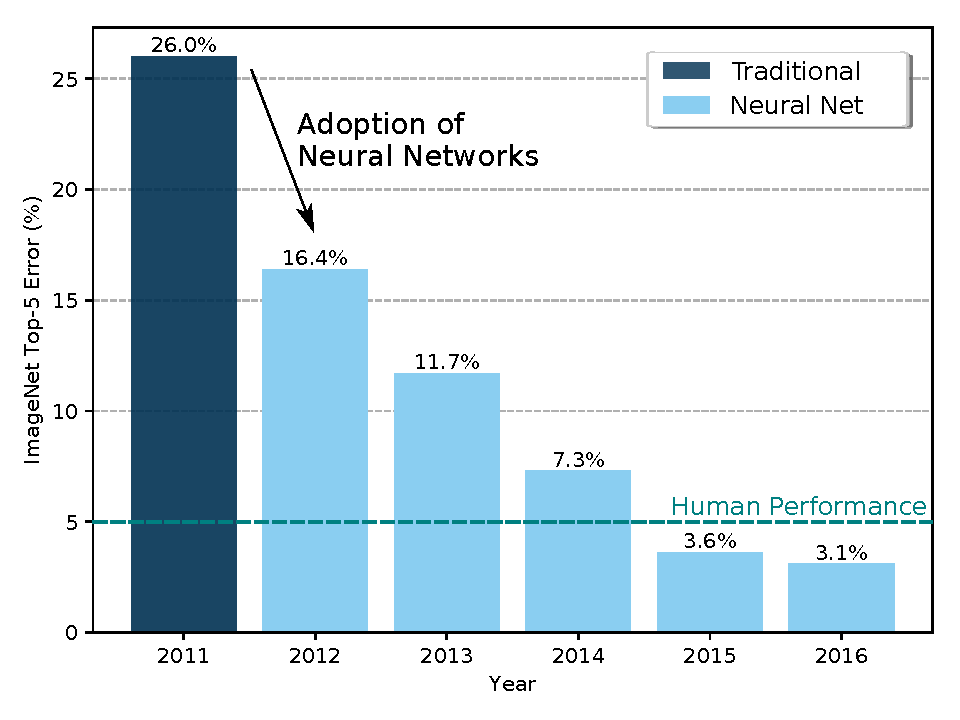
\includegraphics[width=\linewidth]{images/imagenet_results.pdf}
\end{figure}


\end{frame}


\section{Challenges for Deployment}

\subsection{Large Models}

\begin{frame}{Deployment Challenges}

\begin{itemize}
	\item Models are too big for edge devices 
    \item Bottleneck in data movement
    \item Accessing off chip DRAM is expensive in terms of time and energy
\end{itemize}

\end{frame}

\begin{frame}{Parameter Redundancy}



\begin{itemize}
	\item Lucky for us... we know that the vast majority of parameters are redundant 
    \item Many different techniques for compressing networks but the effects are nontrivial
\end{itemize}

\begin{figure}
    \centering
    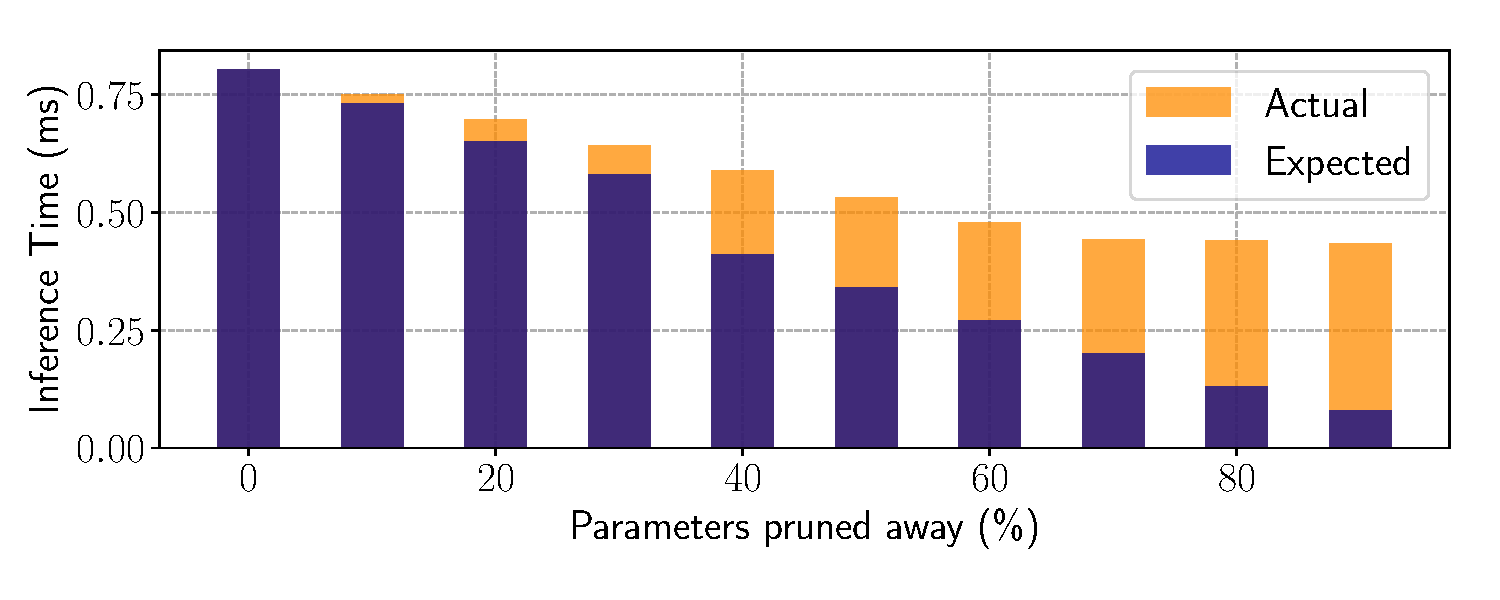
\includegraphics[width=10cm]{images/speedup.pdf}
\end{figure}



\end{frame}


\begin{frame}{Contributions}
    
    \begin{itemize}
        \item Introduction of the \textit{Deep Learning Inference Stack}
        \item Characterisation of various neural network acceleration methods on different hardware
    \end{itemize}
    
\end{frame}


\section{Background}

\begin{frame}{Background: Neurons}

\begin{figure}
    \centering
    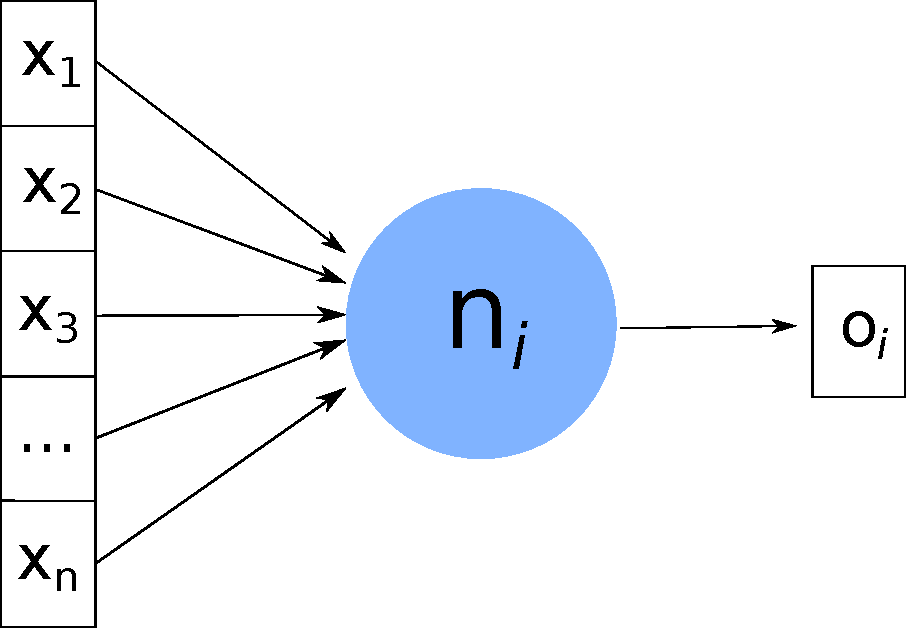
\includegraphics[width=0.8\textwidth]{images/neuron.pdf}
\end{figure}

\end{frame}


\begin{frame}{Background: Affine Transform Neurons}



\end{frame}

\begin{frame}{Background: Convolution Neurons}
\centering
\animategraphics[loop,controls,width=0.6\linewidth]{1}{images/arbitrary_padding_no_strides_0}{0}{3}
\end{frame}

\begin{frame}{Background: Layers}

\begin{figure}
    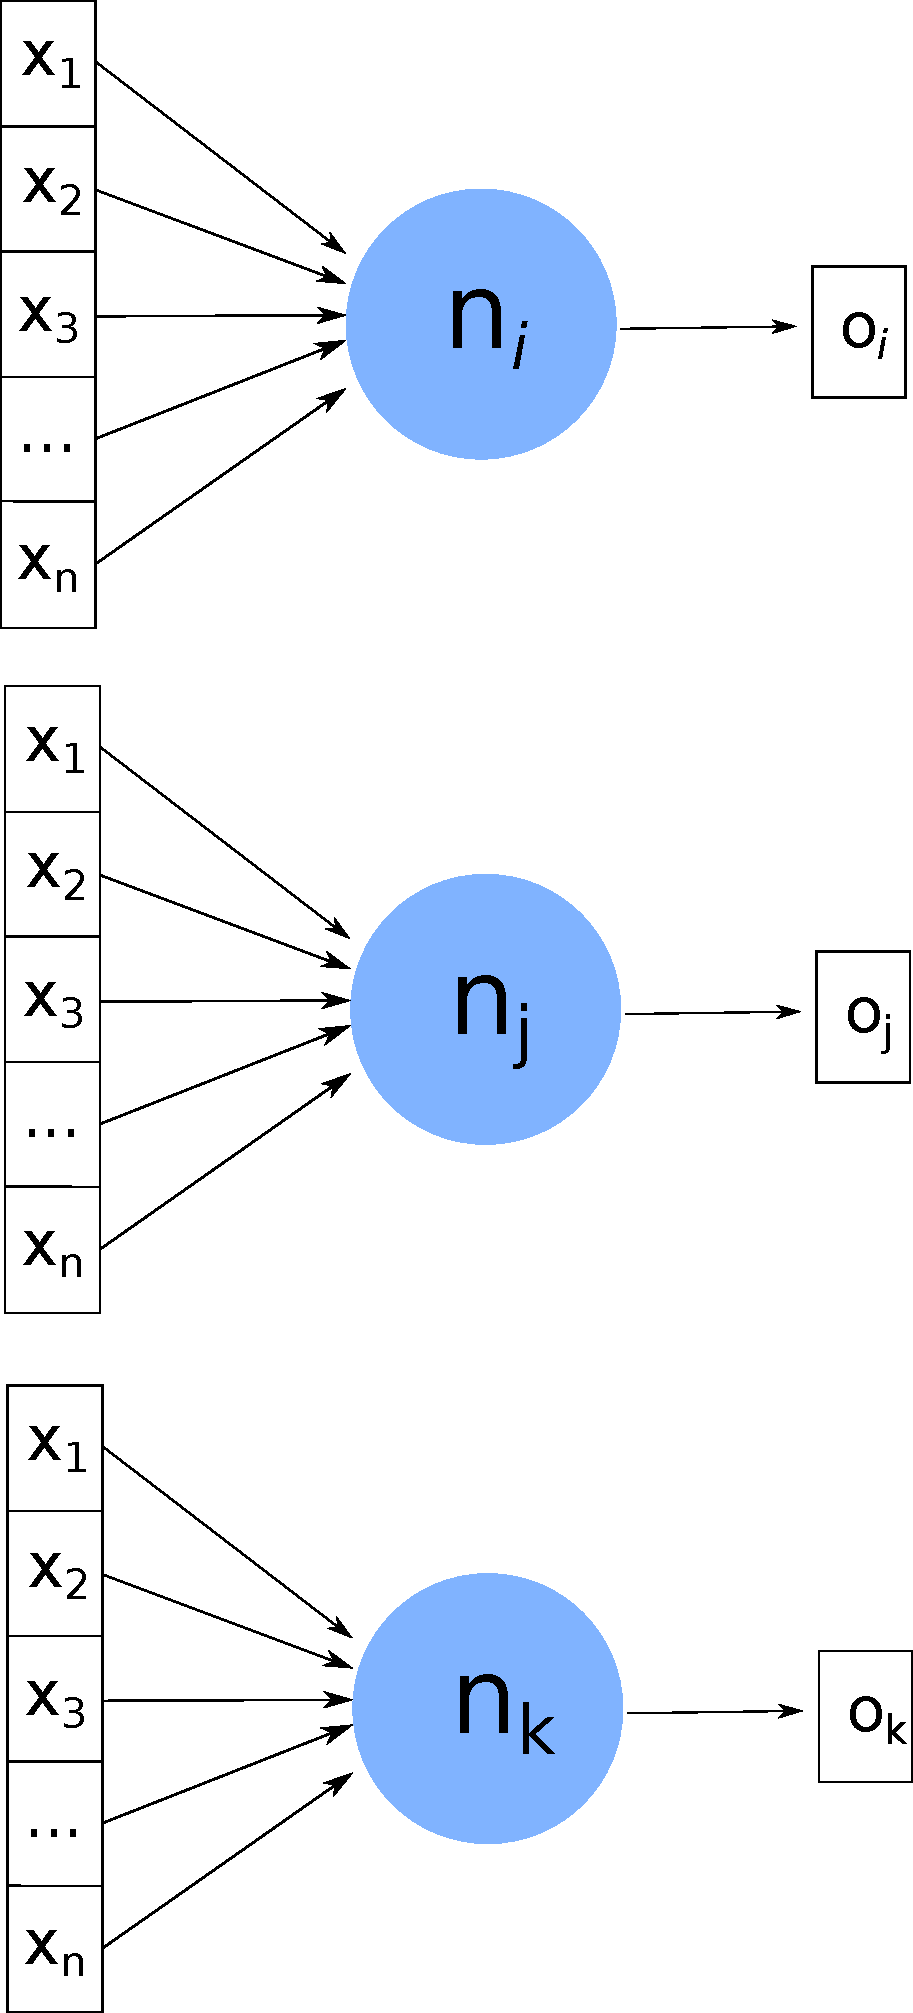
\includegraphics[width=3cm]{images/layer.pdf}
\end{figure}

\end{frame}


\begin{frame}{Background: Neural Networks}

\begin{figure}
    \centering
    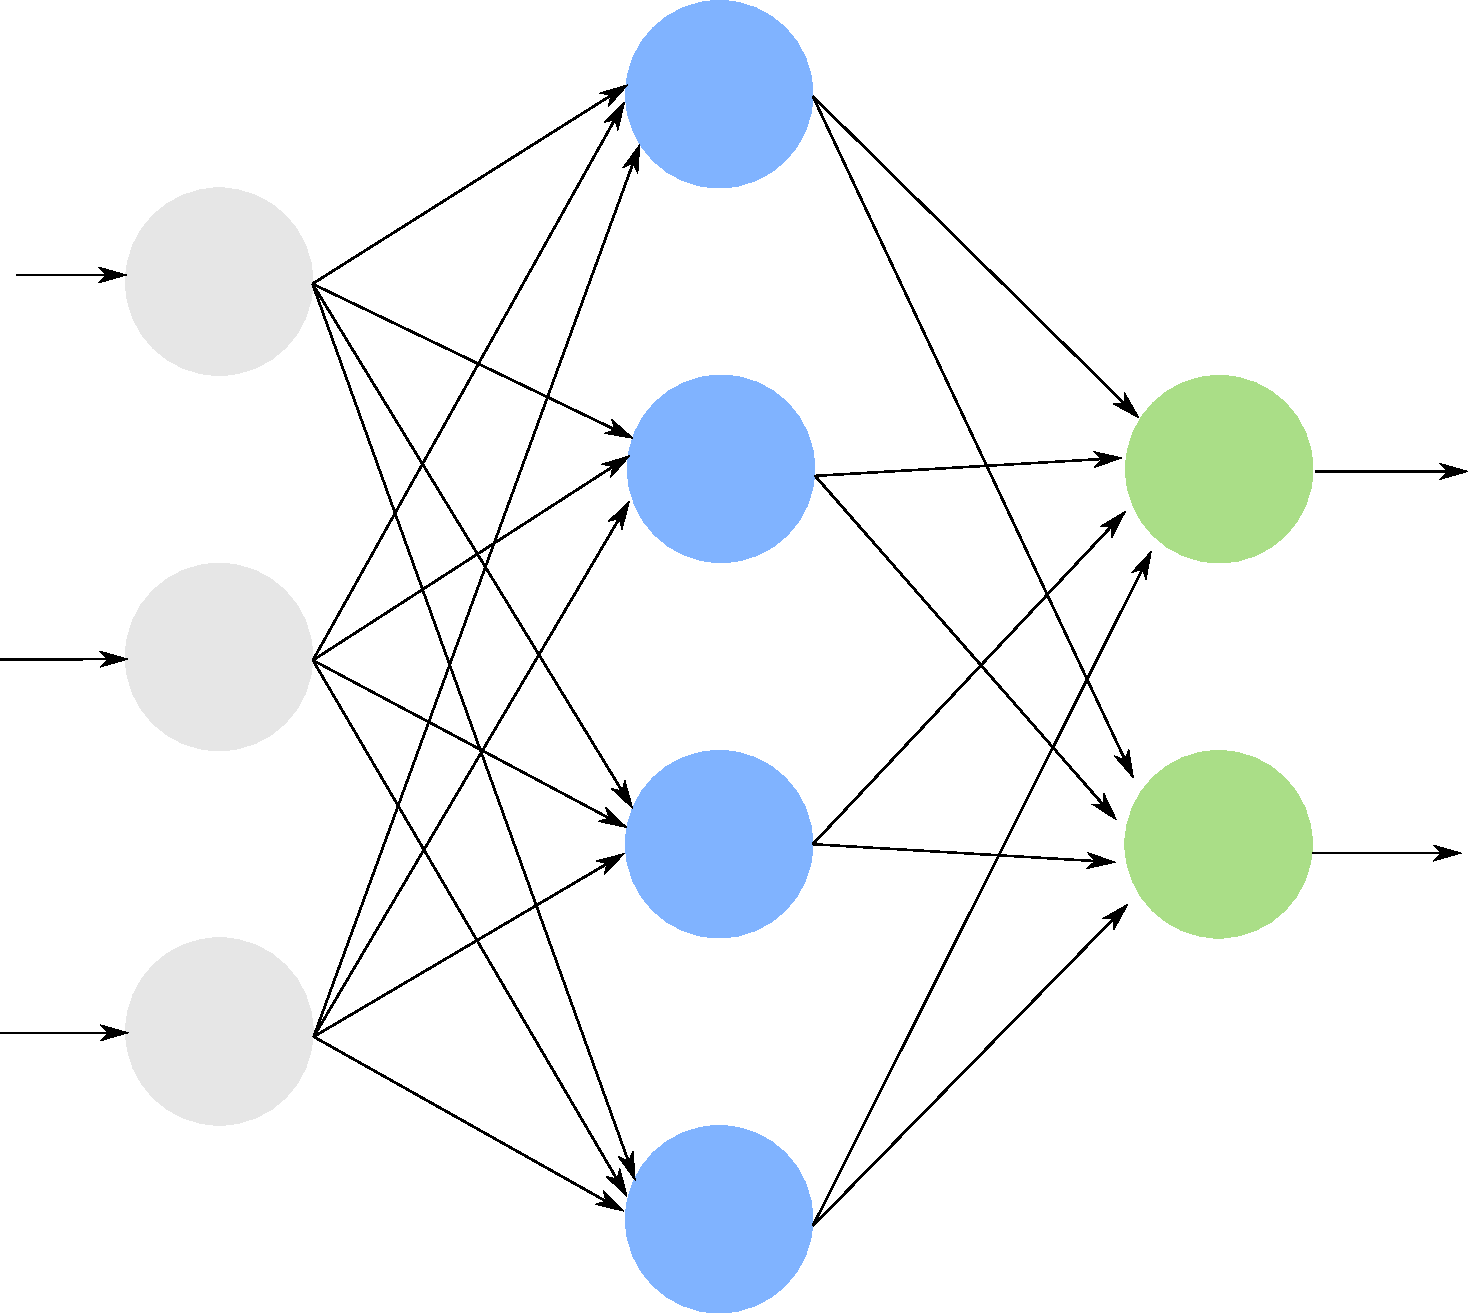
\includegraphics[width=0.6\linewidth]{images/neural_network.pdf}
\end{figure}
\end{frame}



\begin{frame}{Background: Weight Pruning}

\begin{itemize}
    \item Pruning at the individual \textit{weight} level
    \item Leaves weight matrices very sparse
\end{itemize}

\begin{figure}
    \centering
    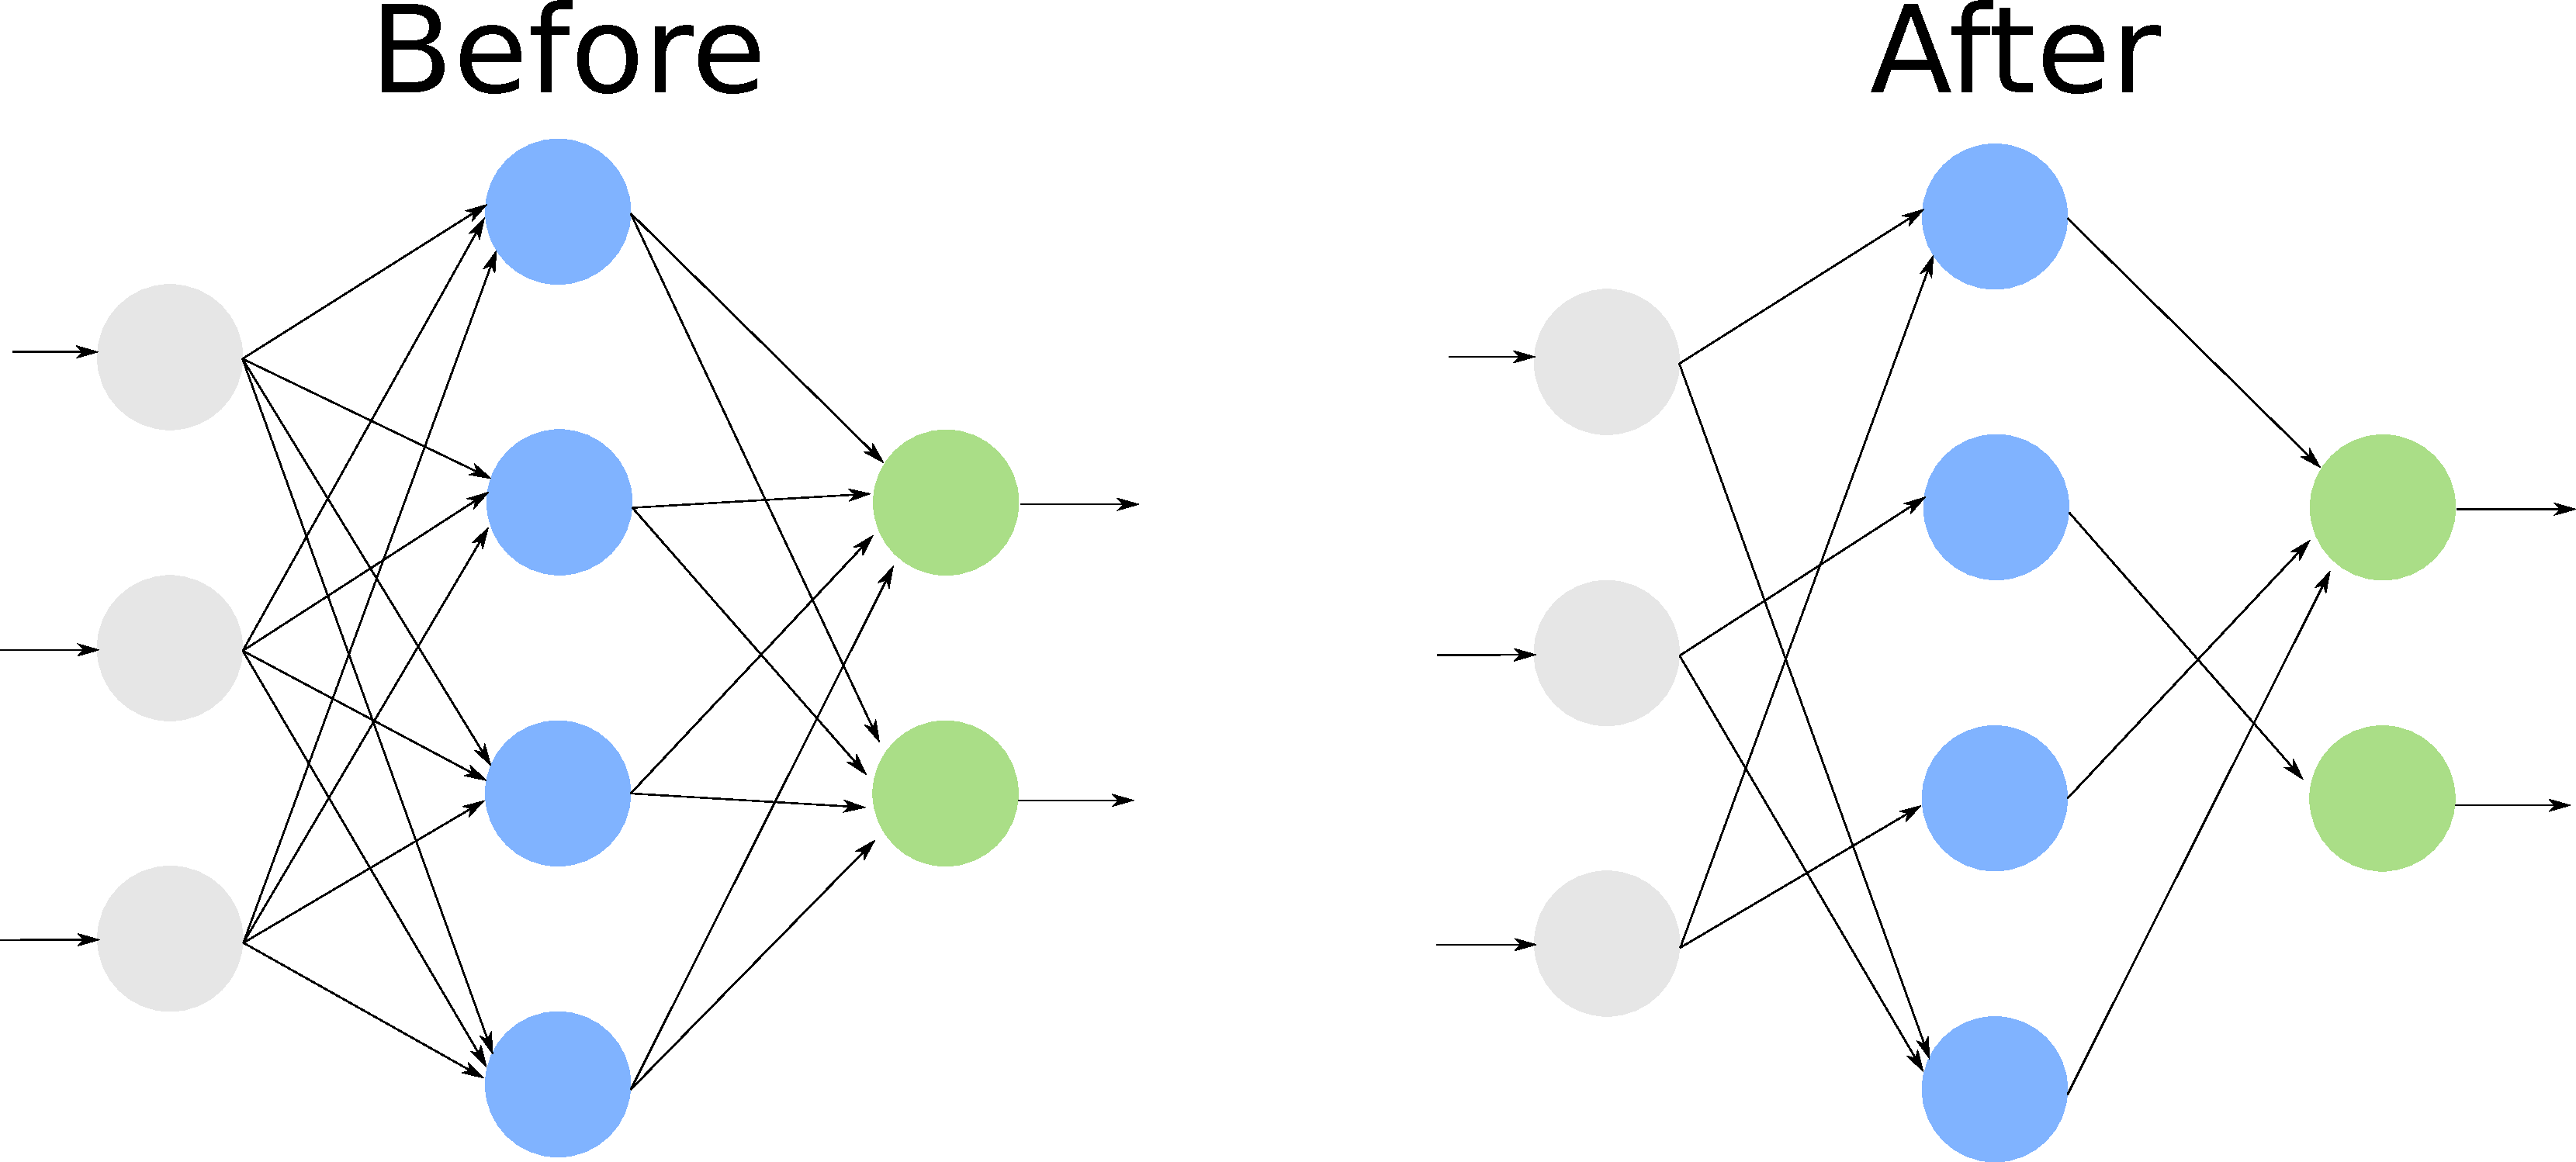
\includegraphics[width=8cm]{images/weight_pruning.pdf}
\end{figure}

\end{frame}


\begin{frame}{Background: Channel Pruning}

\begin{itemize}
    \item Pruning at the \textit{neuron} level
    \item Leaves weight matrices small and dense
\end{itemize}

\begin{figure}
    \centering
    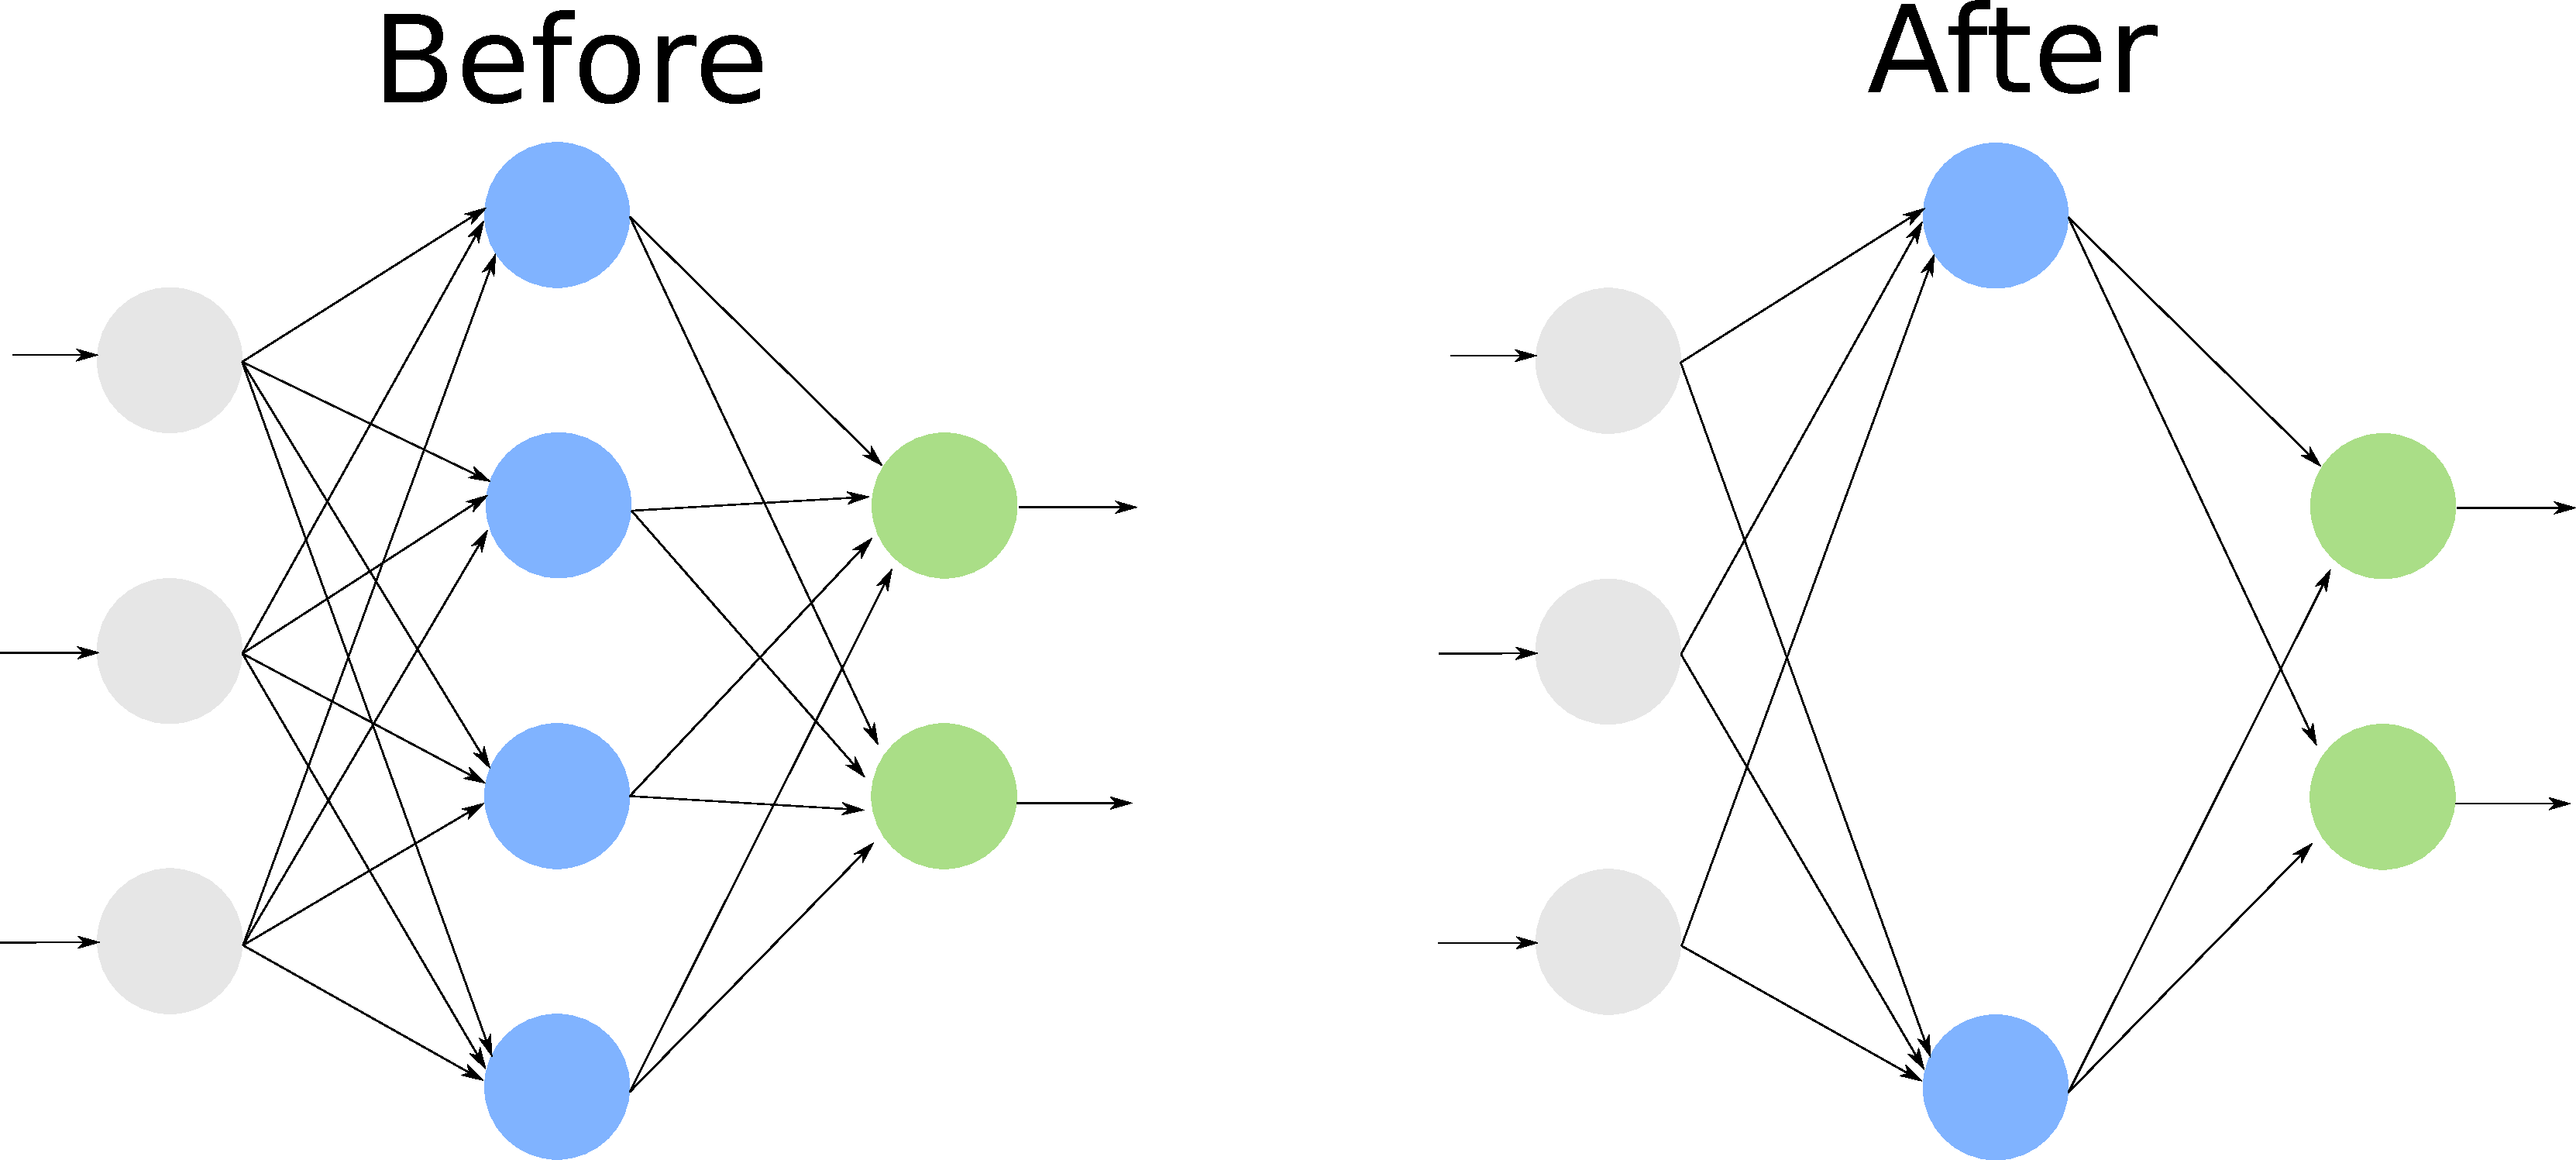
\includegraphics[width=8cm]{images/channel_pruning.pdf}
    \label{fig:channel_pruning}
\end{figure}

\end{frame}


\begin{frame}{Background: Quantisation}
\begin{itemize}
    \item Two options:
    \begin{enumerate}
        \item Reduce precision of weights
        \item Group to small set of centroids
    \end{enumerate}
\end{itemize}

\begin{figure}
    \centering
    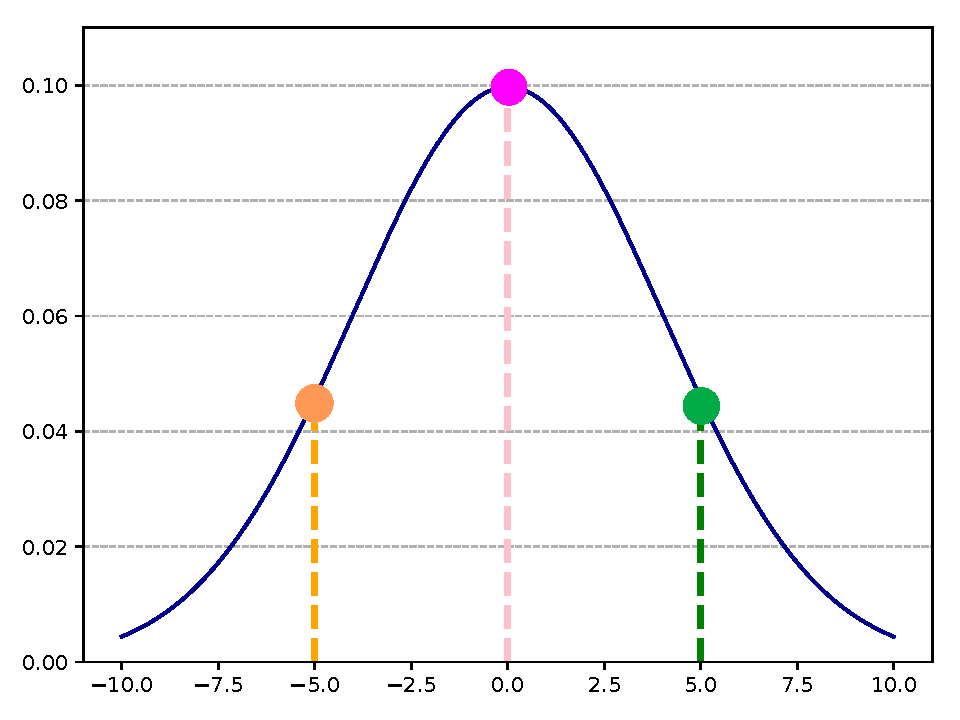
\includegraphics[width=5cm]{images/quantization.pdf}
\end{figure}


\end{frame}


\section{Inference Stack}

\begin{frame}{The Deep Learning Inference Stack}
\begin{figure}
    \centering
    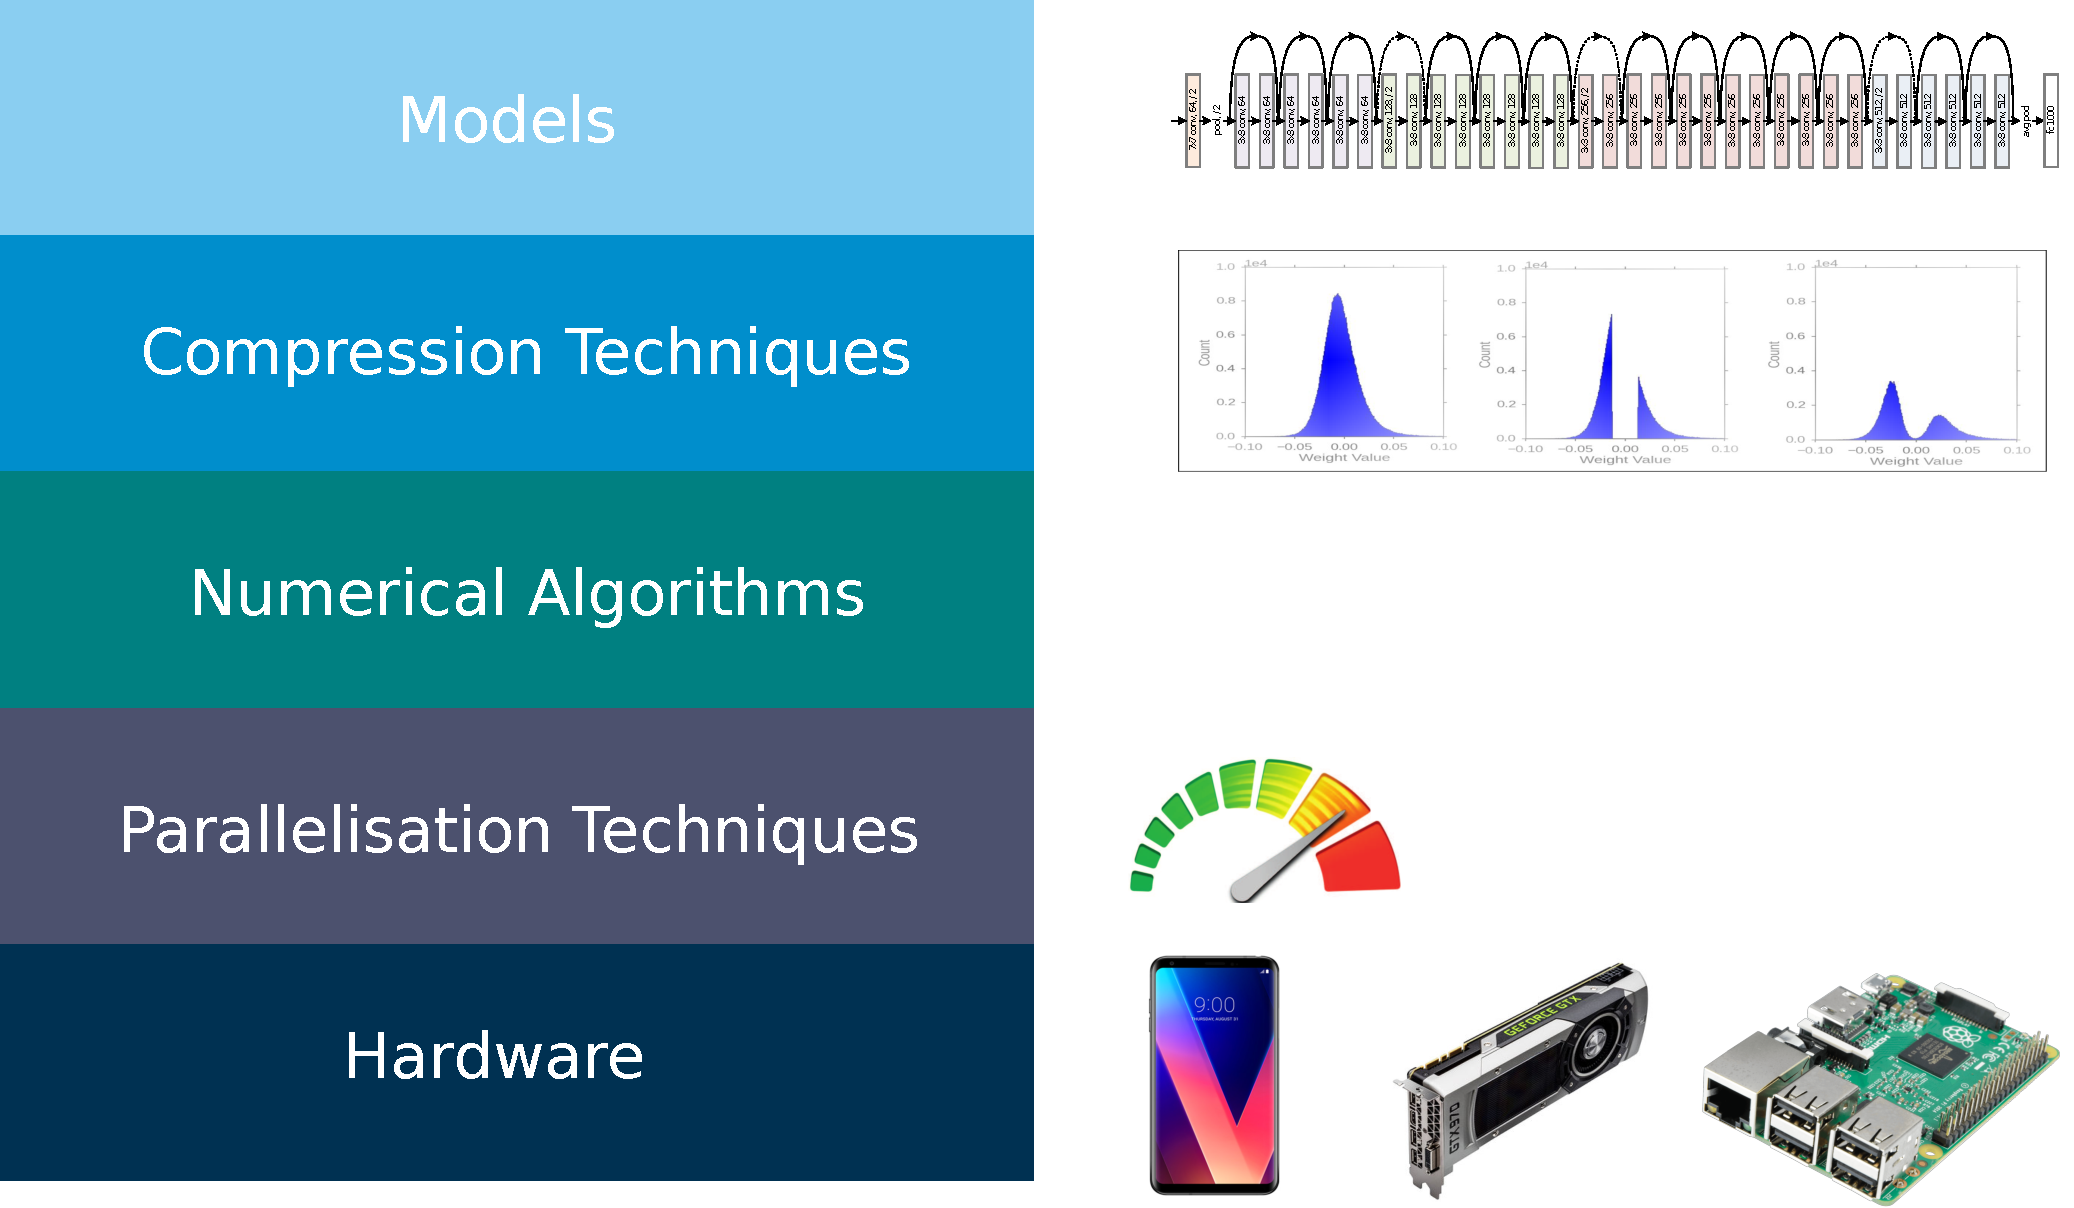
\includegraphics[width=\linewidth]{images/inference-stack.pdf}
    \caption{The Deep Learning Inference Stack}
    \label{fig:inference-stack}
\end{figure}
\end{frame}

\begin{frame}{Layer 1: Neural Networks}

\begin{columns}
\column{0.3\textwidth}

\begin{figure}
    \centering
    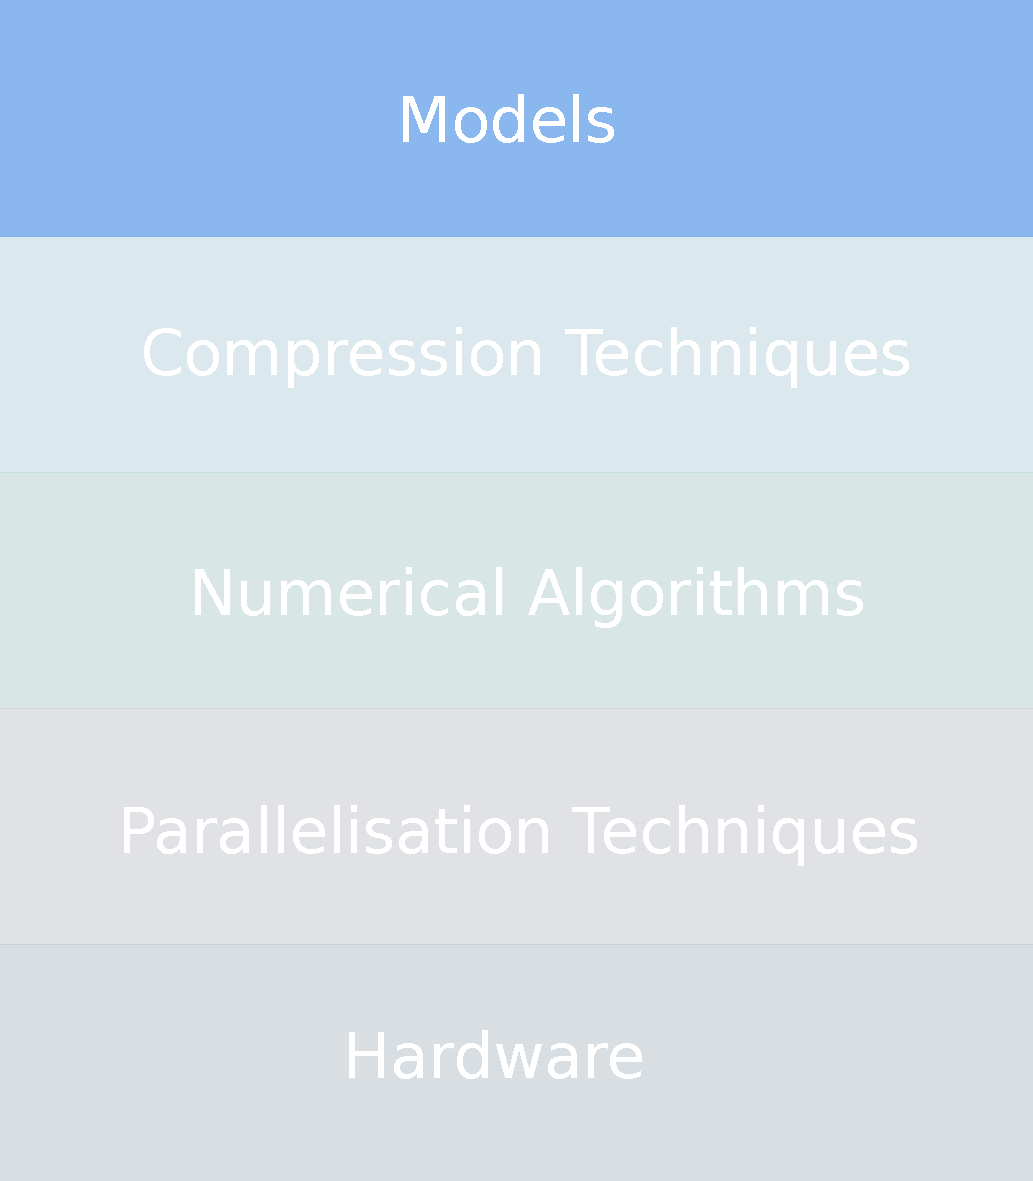
\includegraphics[width=3.5cm]{images/models.pdf}
    \label{fig:inference-stack-models}
\end{figure}

\column{0.7\textwidth}

\textbf{Neural Network Models}

\begin{itemize}
    \item Number of layers
    \item Number of neurons in each layer
    \item Operation each neuron performs
\end{itemize}

\begin{figure}
    \centering
    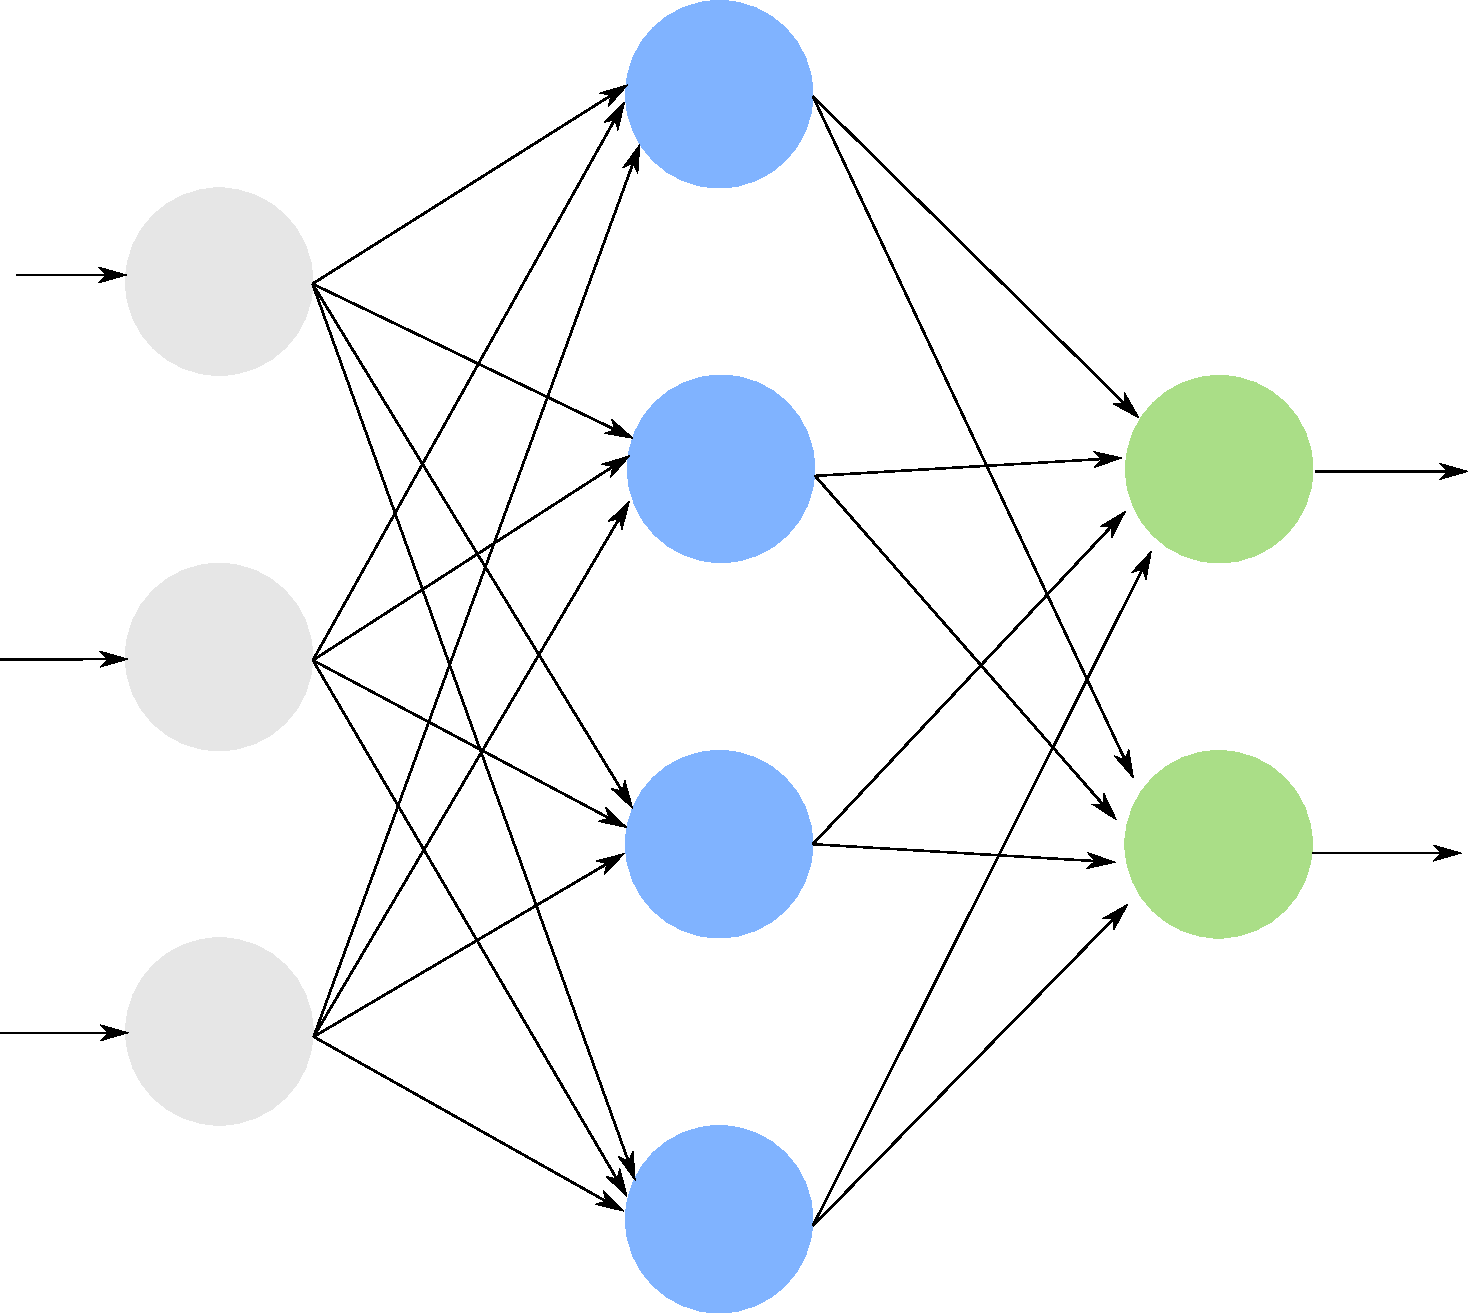
\includegraphics[width=5.5cm]{images/neural_network.pdf}
\end{figure}

\end{columns}


\end{frame}

\definecolor{bg}{rgb}{0.95,0.95,0.95}

\begin{frame}{Layer 1: Neural Networks}
\vspace{0.2cm}

\inputminted[bgcolor=bg, fontfamily=cmss]{python}{images/mini_model.py}

\begin{figure}
    \centering
    \vspace{-1cm}
    
\includegraphics[width=10cm]{images/lgoos.pdf}
\end{figure}
\end{frame}


\begin{frame}{Layer 1: Neural Networks}
\vspace{0.2cm}

\begin{itemize}
    \item VGG-16
    \item MobileNet
    \item ResNet-18
\end{itemize}

\end{frame}


\begin{frame}{Layer 2: Compression Techniques}

\begin{columns}
\column{0.3\textwidth}
\begin{figure}
    \centering
    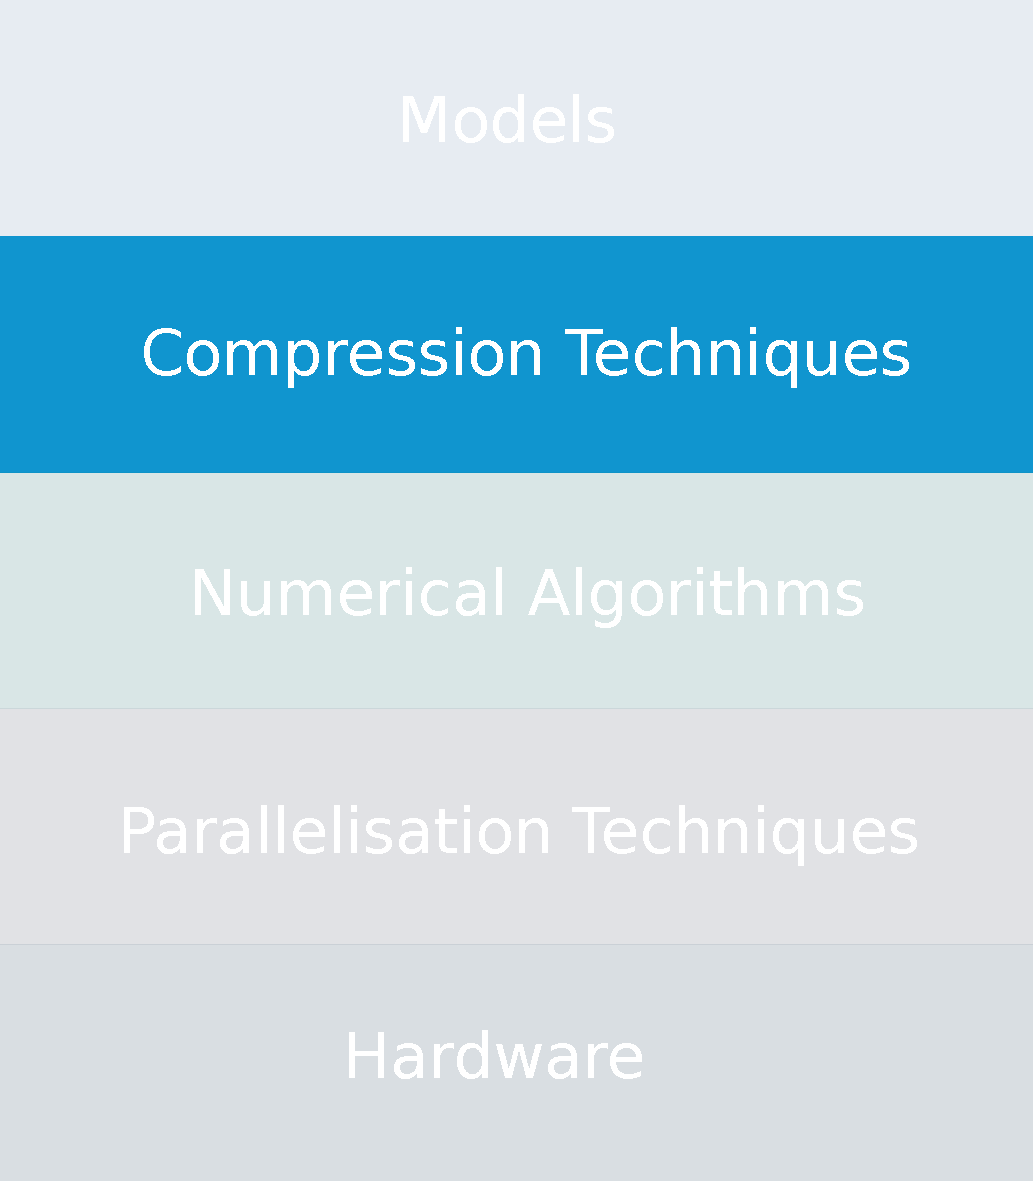
\includegraphics[width=3.5cm]{images/compressions.pdf}
    \label{fig:inference-stack-compress-1}
\end{figure}

\column{0.7\textwidth}

\begin{enumerate}
    \item Weight Pruning
    \item Channel Pruning
    \item Quantisation
\end{enumerate}


\end{columns}

\end{frame}



\begin{frame}{Layer 2: Weight Pruning}

\begin{itemize}
    \item Deep compression
    \item Magnitude based thresholding 
    \item Iterate over steps of sparsifying and retraining 
    \item Leave the matrices very sparse but get up to 90\% compression rate
\end{itemize}
    
\end{frame}


\begin{frame}{Layer 2: Channel Pruning}
    
\begin{itemize}
    \item Fisher pruning
    \item Taylor expansion of the objective
    \item Weighted with a FLOP penalty $\beta$
\end{itemize}
    
\end{frame}


\begin{frame}{Layer 2: Quantisation}
\begin{itemize}
    \item TTQ
    \item Similar thresholding concept to weight pruning
    \item Group to a set of three values 
    \item Inference can be done with just these three values
    \item Often also have some sparsity (since one of the three values is zero)
\end{itemize}
    
\end{frame}


\begin{frame}{Layer 3: Numerical Algorithms}

\begin{columns}

\column{0.3\textwidth}
\begin{figure}
    \centering
    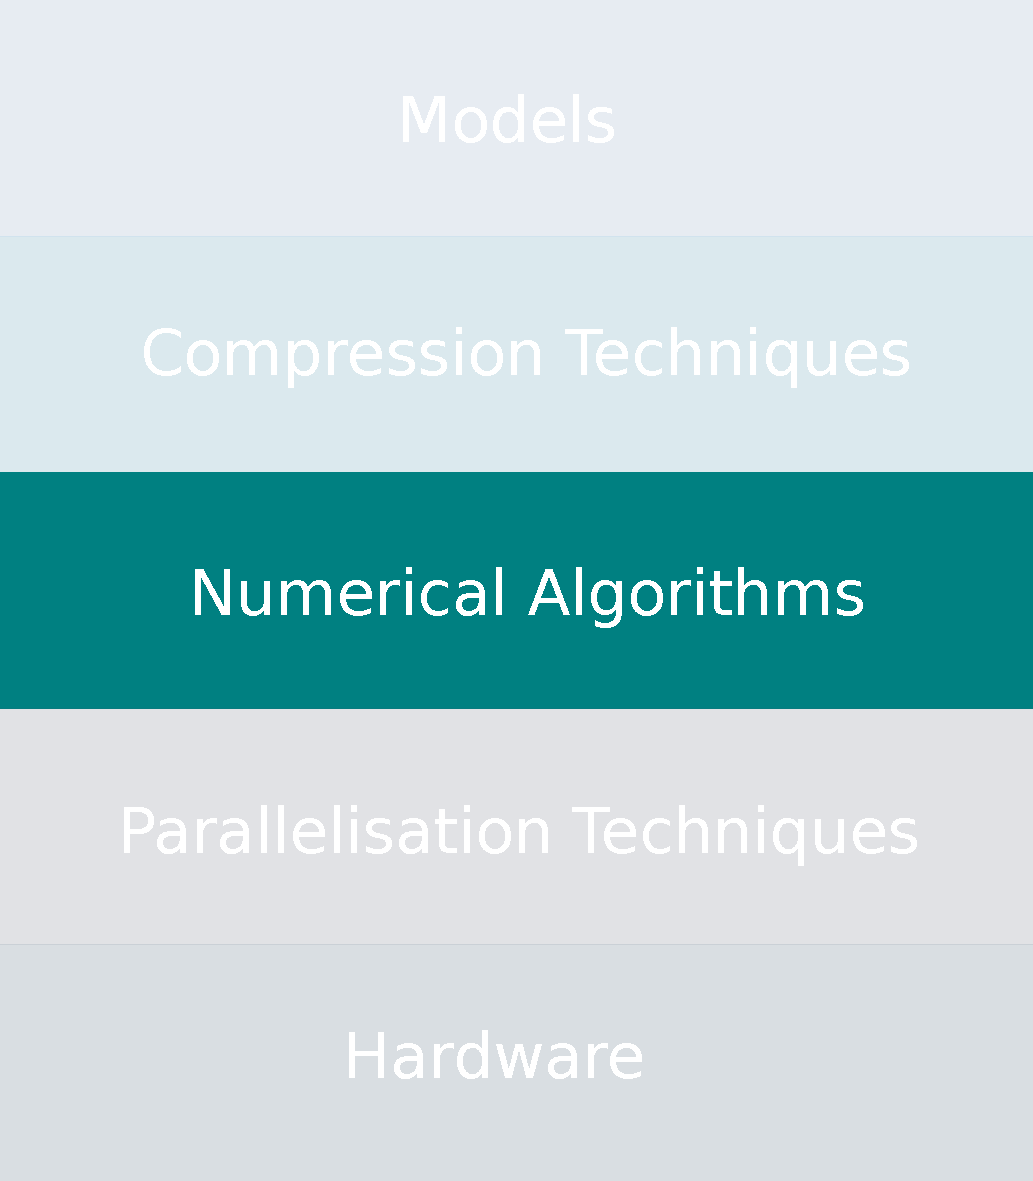
\includegraphics[width=3.5cm]{images/numericals.pdf}
    \label{fig:inference-stack-nums-1}
\end{figure}

\column{0.7\textwidth}

\begin{itemize}
    \item Direct convolution
    \item \texttt{im2col}
    \item FFT and Winograd
\end{itemize}

\end{columns}
\end{frame}


\begin{frame}{Layer 3: Numerical Algorithms}

\begin{columns}

\column{0.3\textwidth}

\begin{figure}
    \centering
    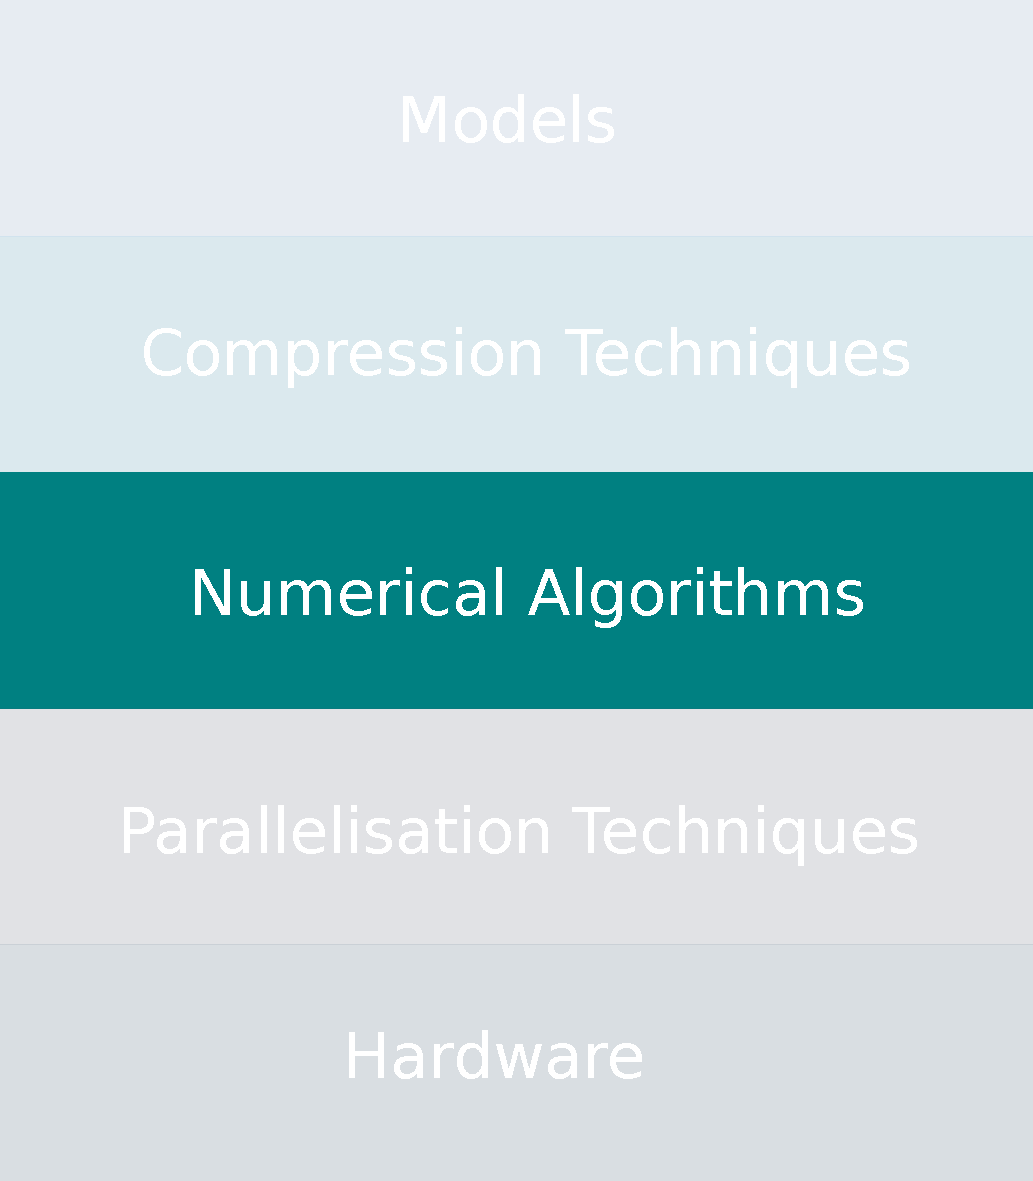
\includegraphics[width=3.5cm]{images/numericals.pdf}
    \label{fig:inference-stack-nums-2}
\end{figure}

\column{0.7\textwidth}
\begin{itemize}
    \item CSR
\end{itemize}

\end{columns}
\end{frame}

\begin{frame}{Layer 4: Parallelisation Techniques}

\begin{columns}


\column{0.3\textwidth}
\begin{figure}
    \centering
    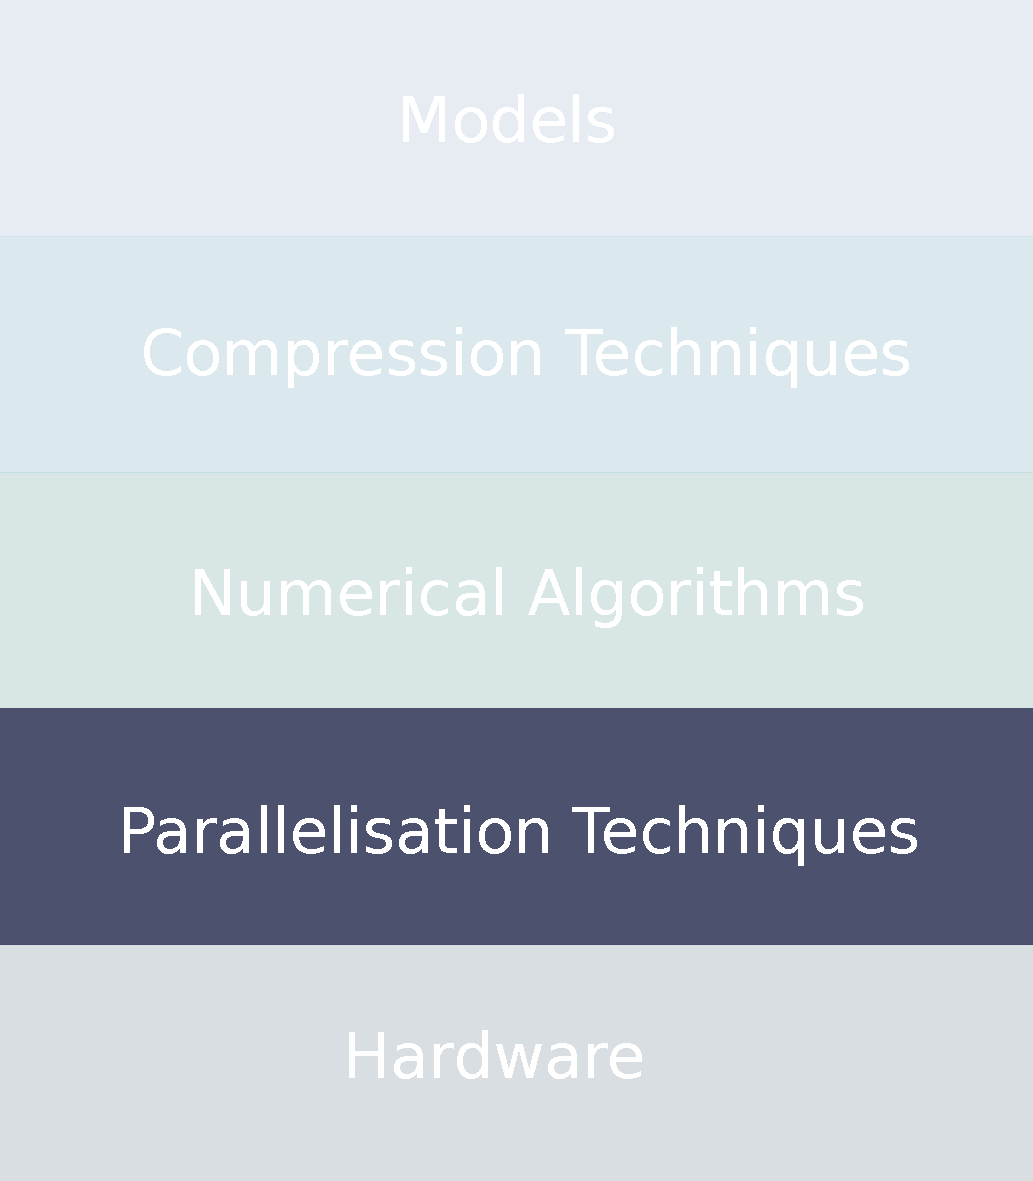
\includegraphics[width=3.5cm]{images/parallelisations.pdf}
    \label{fig:inference-stack-parallels}
\end{figure}

\column{0.7\textwidth}

\textbf{OpenMP}
\begin{itemize}
    \item CPU parallelisation of direct convolution 
    \item Something detailed about how OpenMP handles parallelisation
\end{itemize}

\end{columns}

\end{frame}


\begin{frame}{Layer 4: Parallelisation Techniques}

\begin{columns}


\column{0.3\textwidth}
\begin{figure}
    \centering
    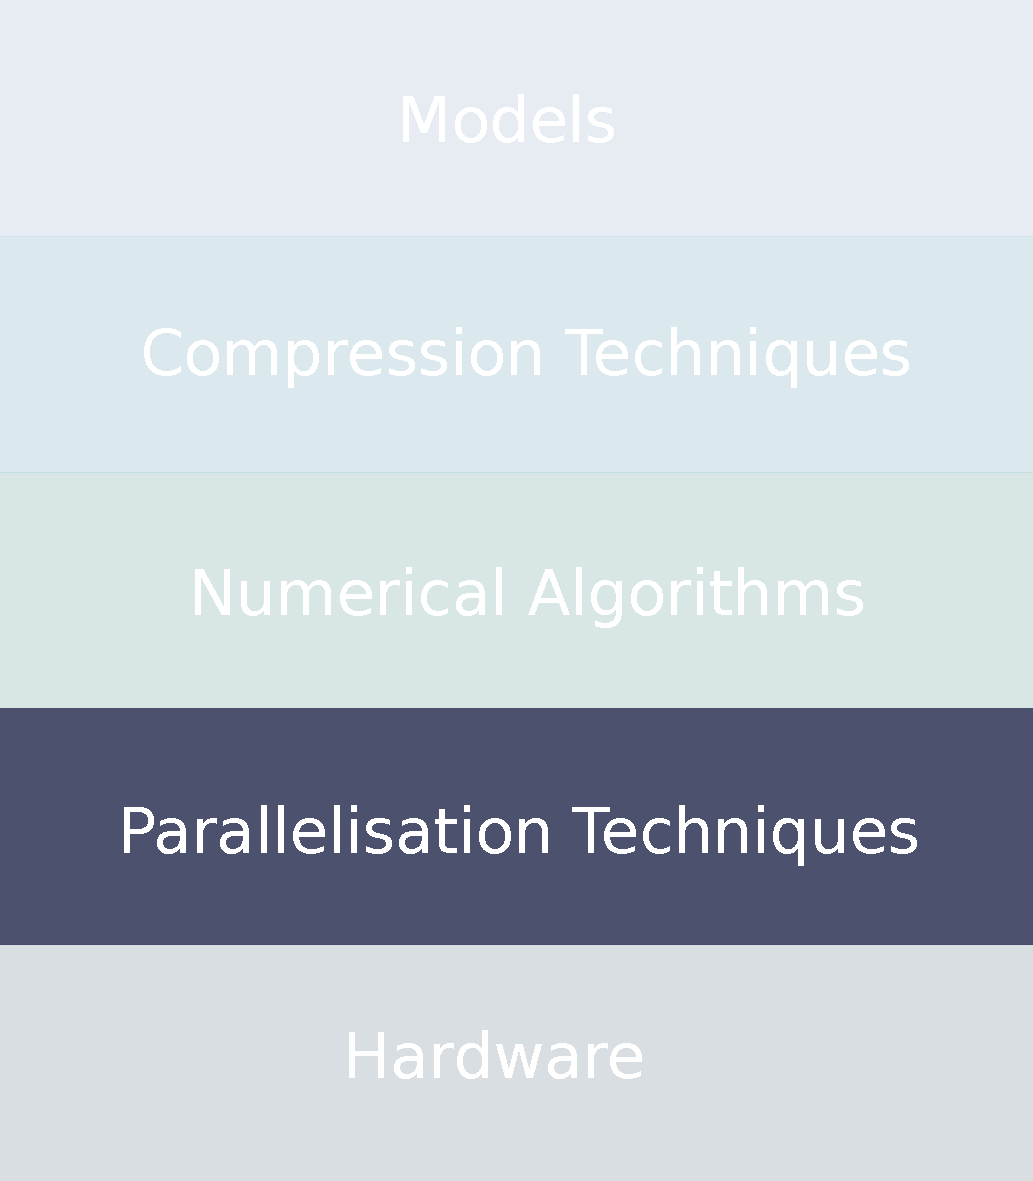
\includegraphics[width=3.5cm]{images/parallelisations.pdf}
    \label{fig:inference-stack-parallels-2}
\end{figure}

\column{0.7\textwidth}

\textbf{OpenCL}
\begin{itemize}
    \item Tile size
    \item Register blocking 
    \item CLBlast Autotuning 
\end{itemize}

\end{columns}

\end{frame}



\begin{frame}{Layer 5: Hardware}

\begin{columns}


\column{0.3\textwidth}
\begin{figure}
    \centering
    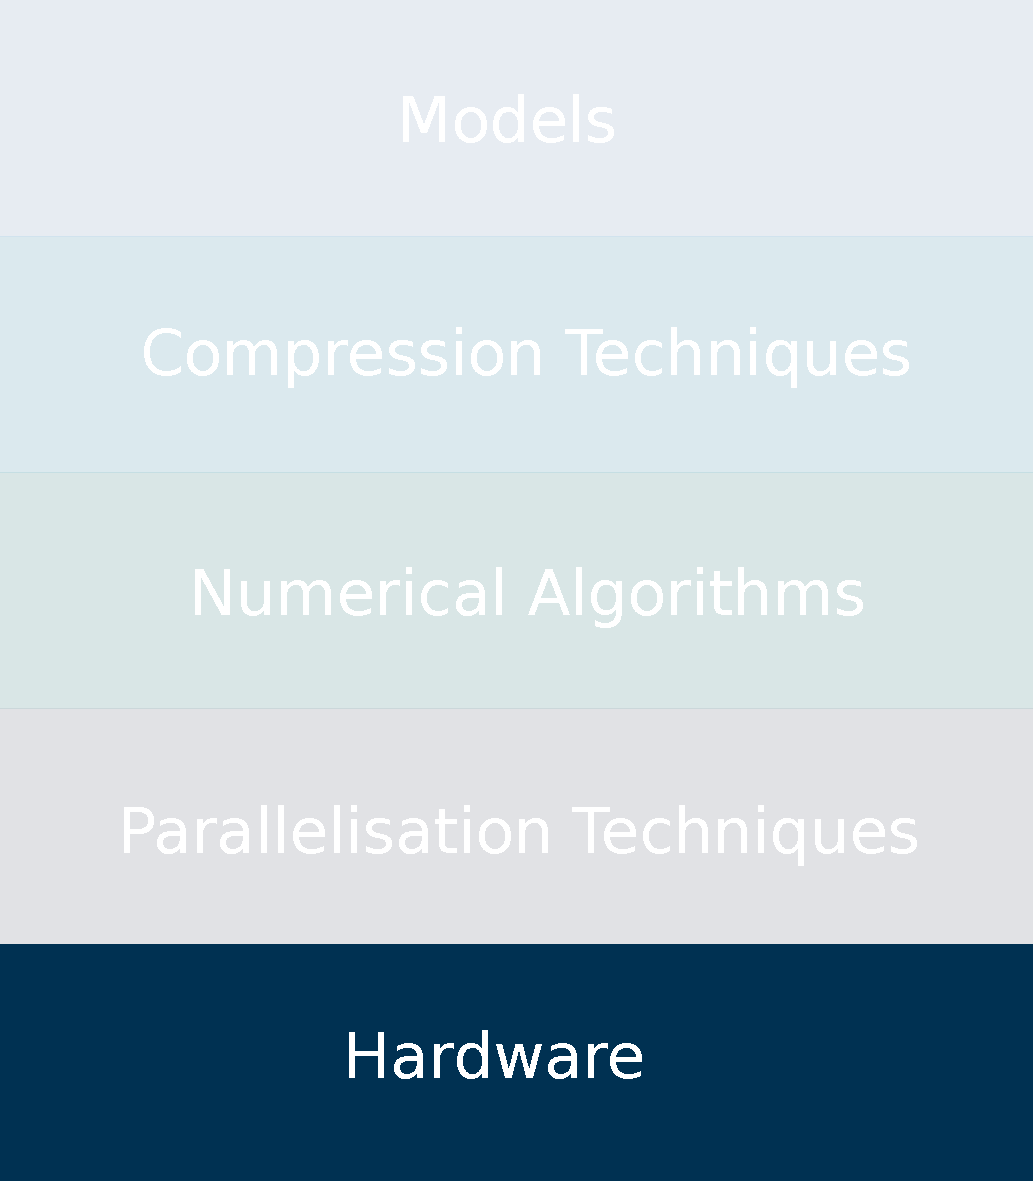
\includegraphics[width=3.5cm]{images/hardwares.pdf}
\end{figure}

\column{0.7\textwidth}

\begin{itemize}
    \item CPU
    \item GPU
    \item Typical embedded device setup
\end{itemize}
\end{columns}


\end{frame}




\section{Experiments}

\begin{frame}{Experiments}

First experiment: take all of the models and apply the compression techniques to them to see their impact on accuracy.
This is good context for the rest of the analysis.
    
\begin{figure}
    \centering
    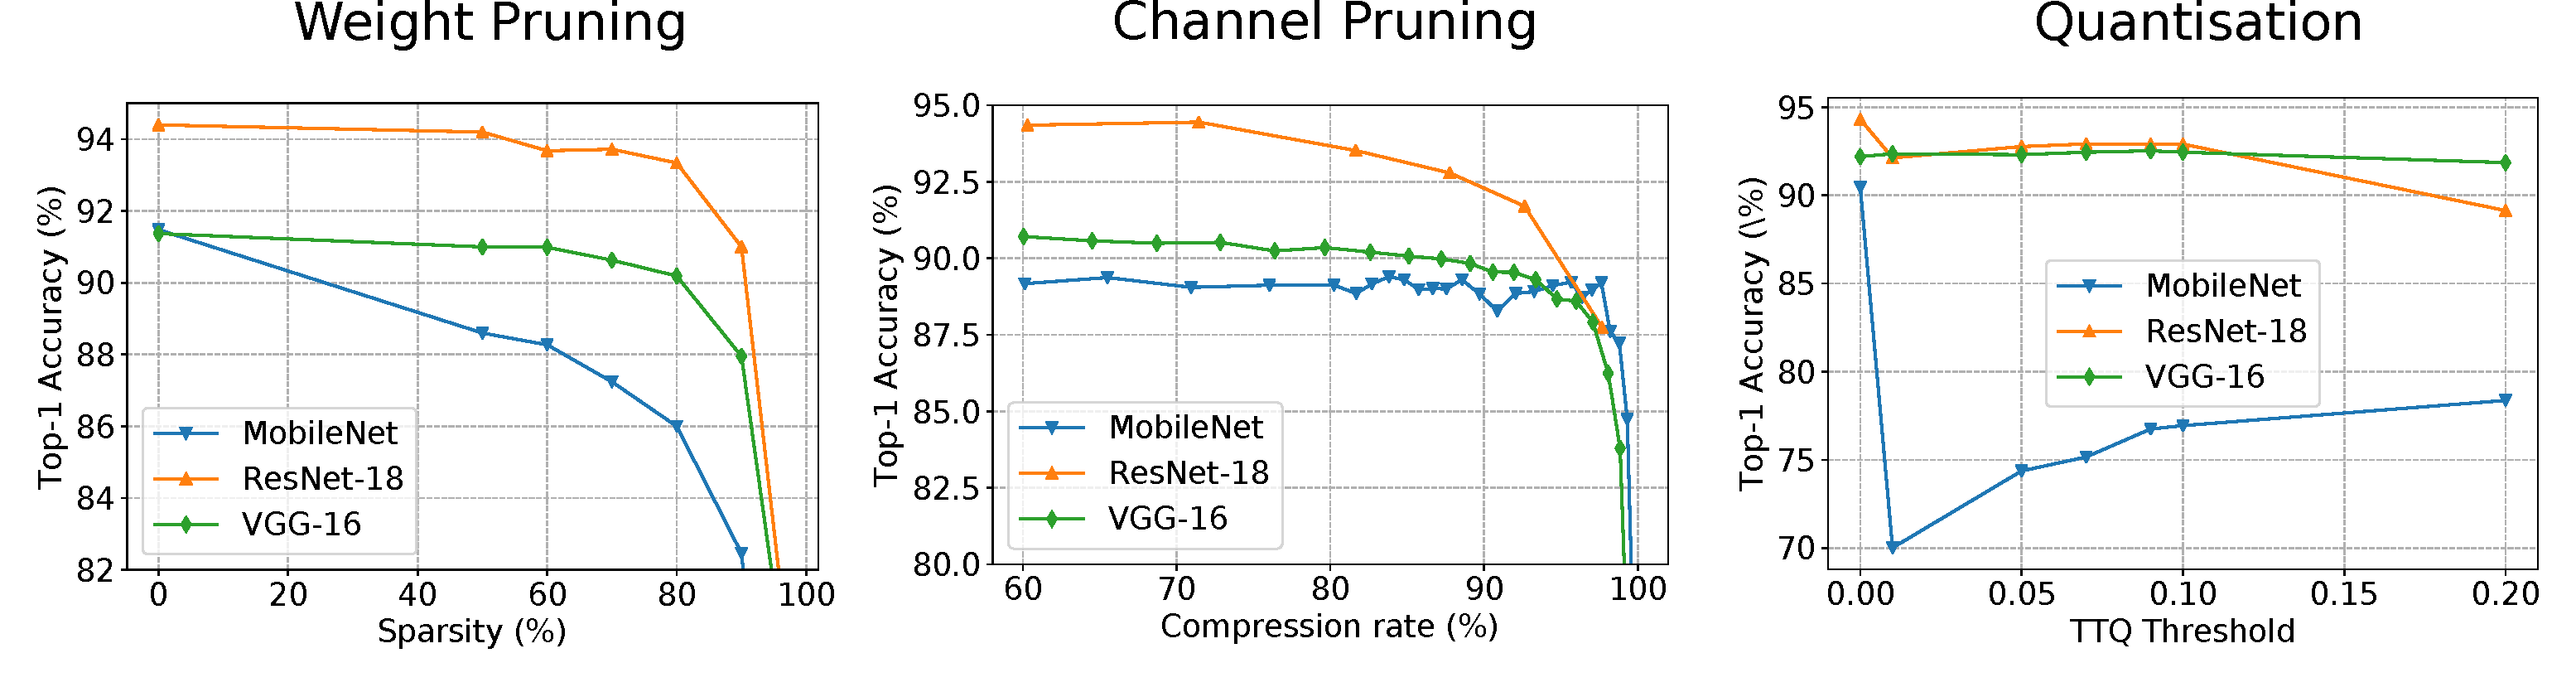
\includegraphics[width=11.75cm]{images/accuracies.pdf}
\end{figure}
    
\end{frame}








{ % all template changes are local to this group.
    \setbeamertemplate{navigation symbols}{}
    \begin{frame}[plain]
        \begin{tikzpicture}[remember picture,overlay]
            \node[at=(current page.center)] {
                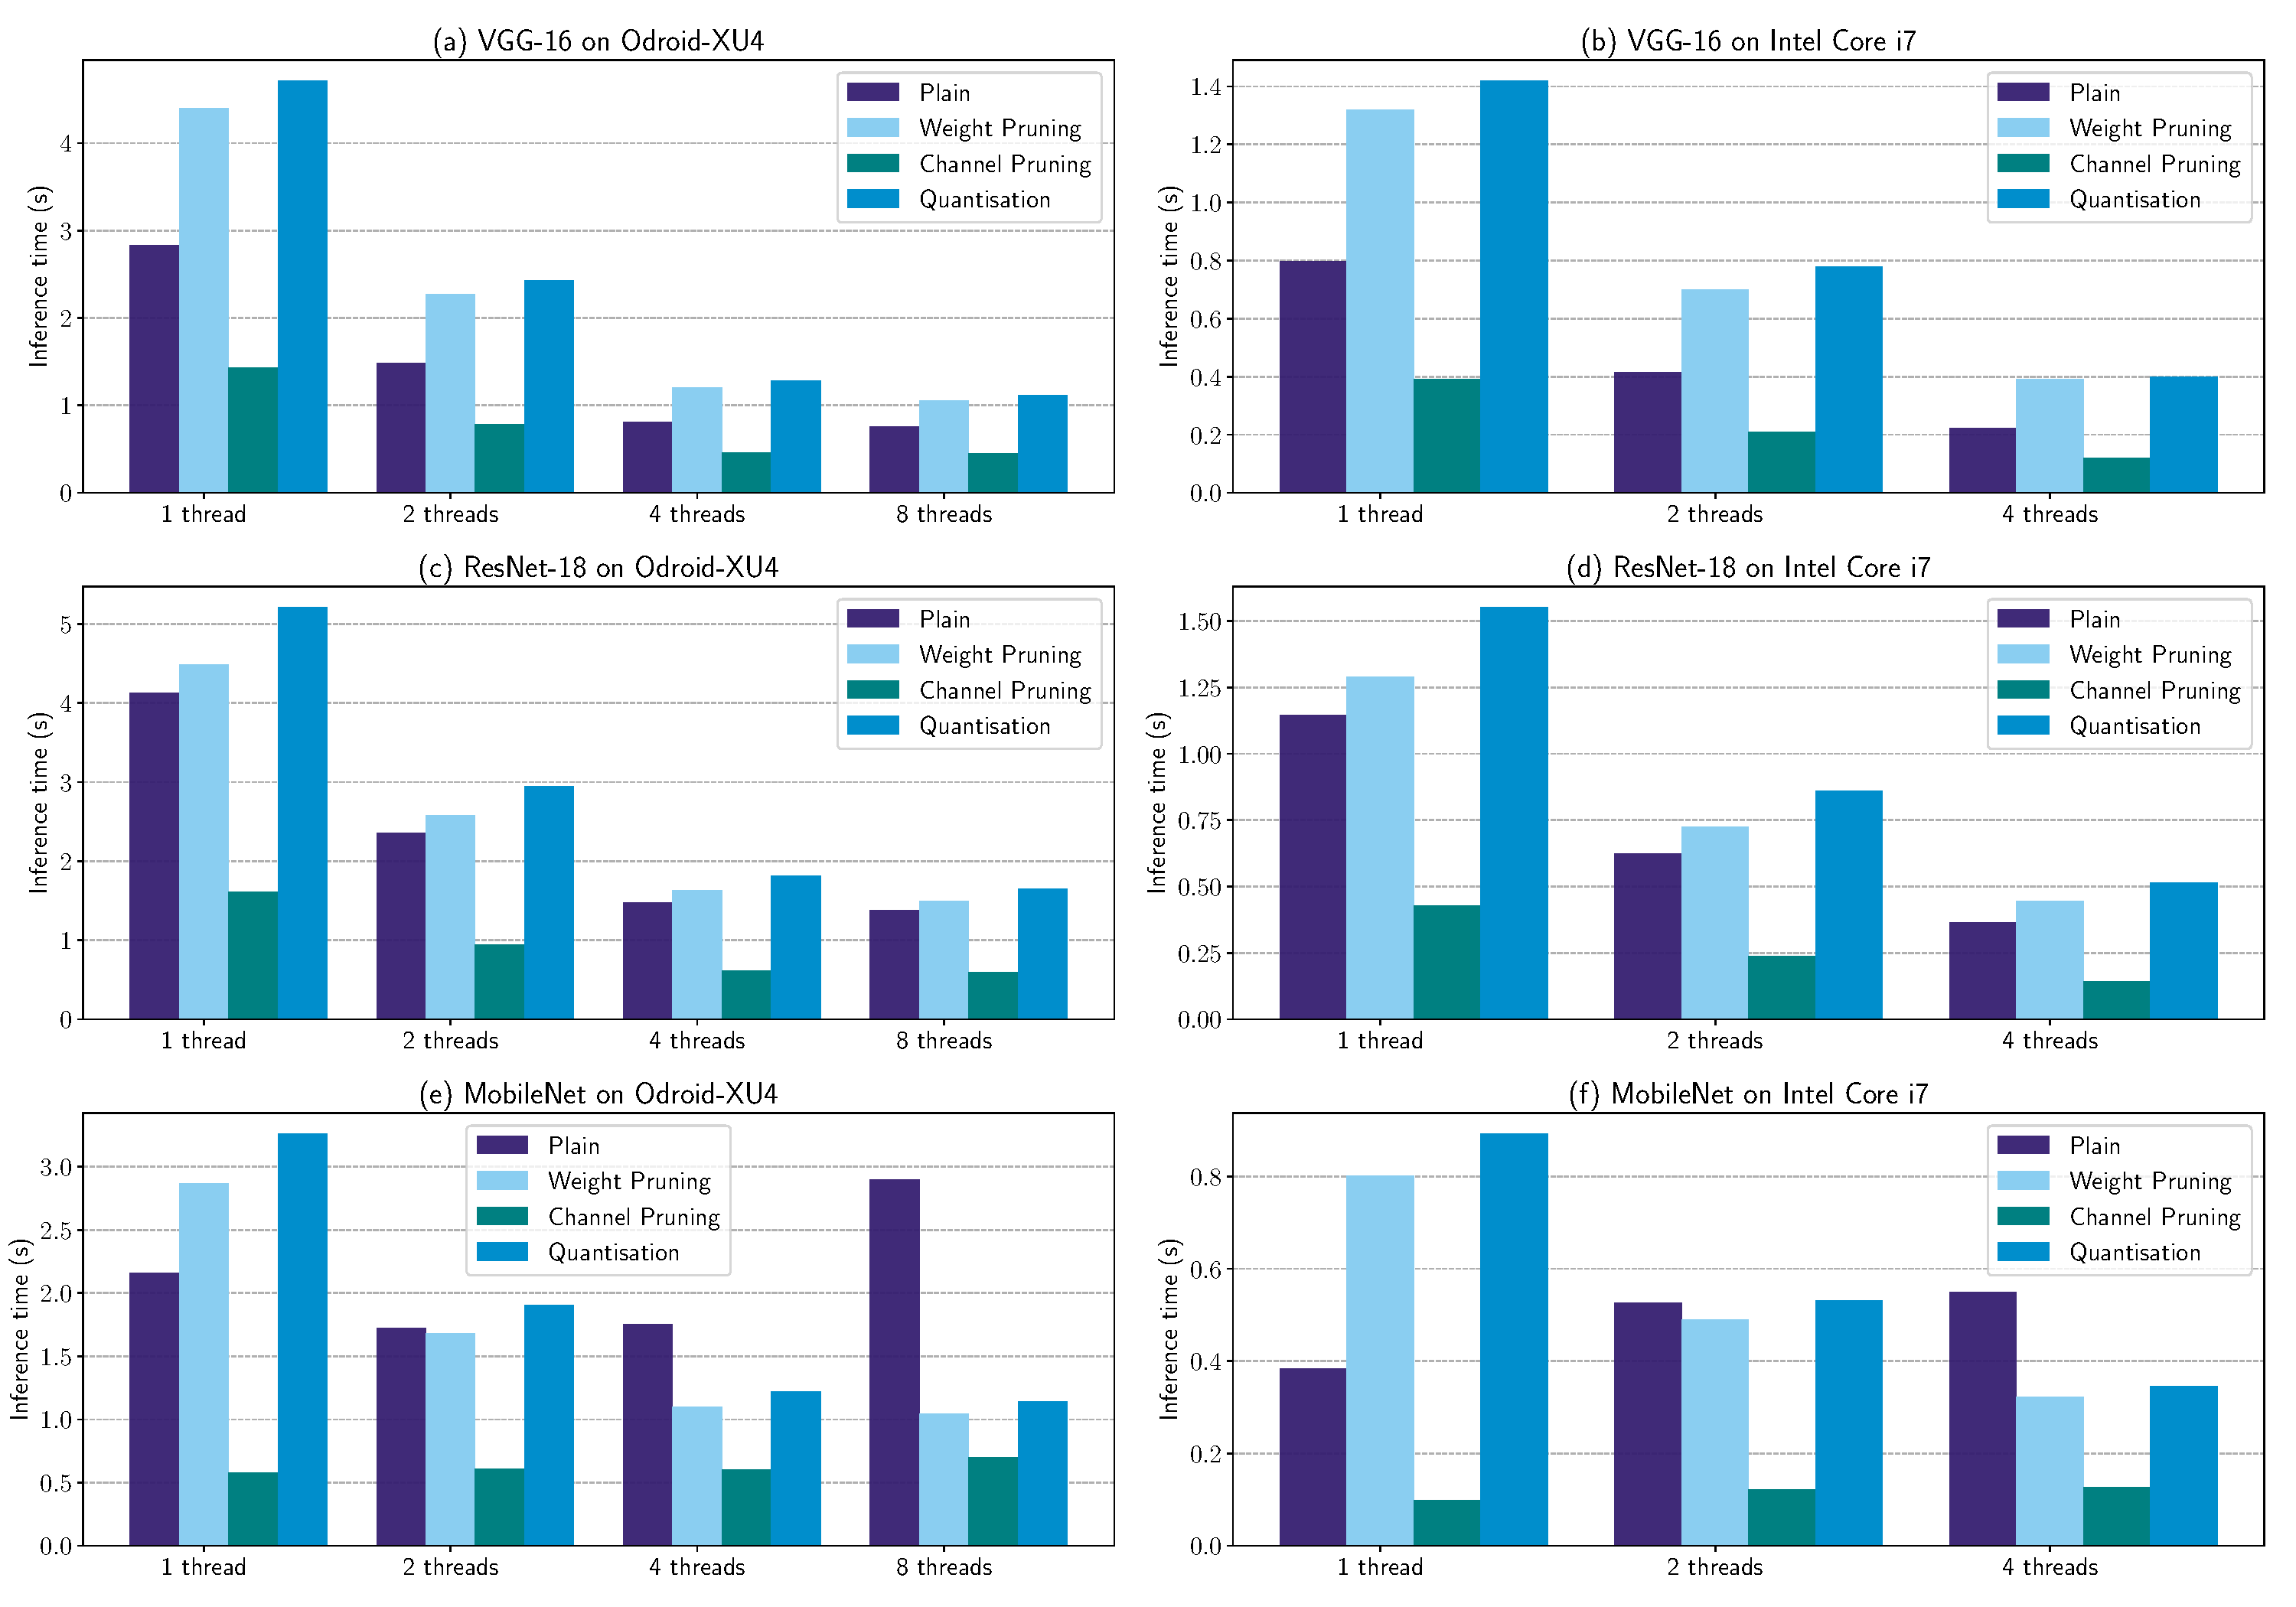
\includegraphics[width=\paperwidth]{images/plots.pdf}
            };
        \end{tikzpicture}
     \end{frame}
}











\begin{frame}{Experiments}
    
Show threading effect is the same on both devices 
    
\end{frame}







\begin{frame}{Experiments}

Show threading MobileNet slows it down.
    
\end{frame}



\begin{frame}{Experiments}
    
    \begin{figure}
        \centering
        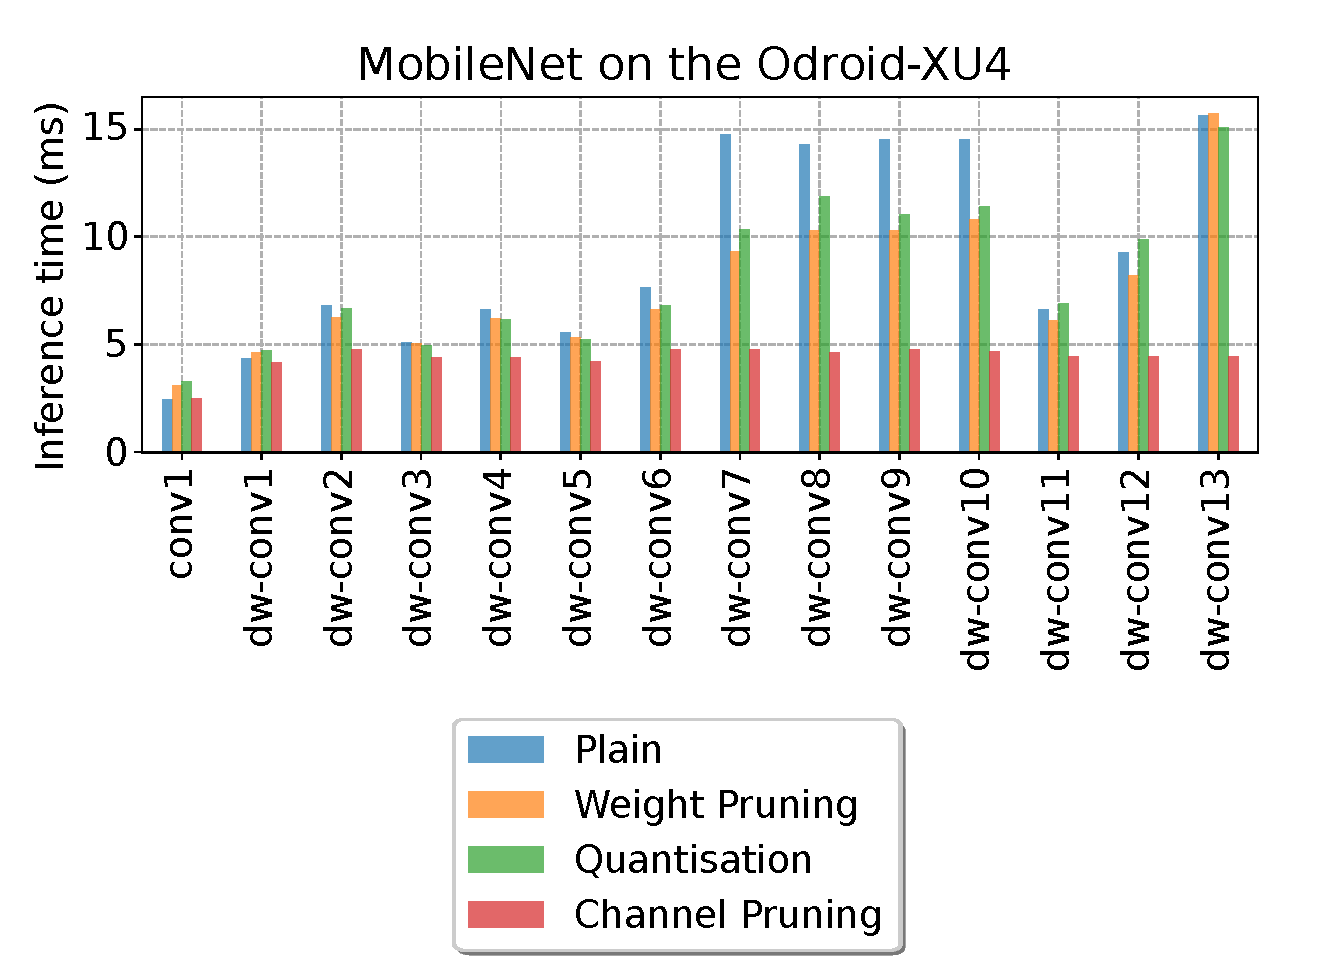
\includegraphics[width=11cm]{images/mobilenet-odroid.pdf}
    \end{figure}
    
\end{frame}


\begin{frame}{Experiments}
    
    Now fix the accuracy at 90\% to make results more comparable.
    
    \begin{figure}
        \centering
        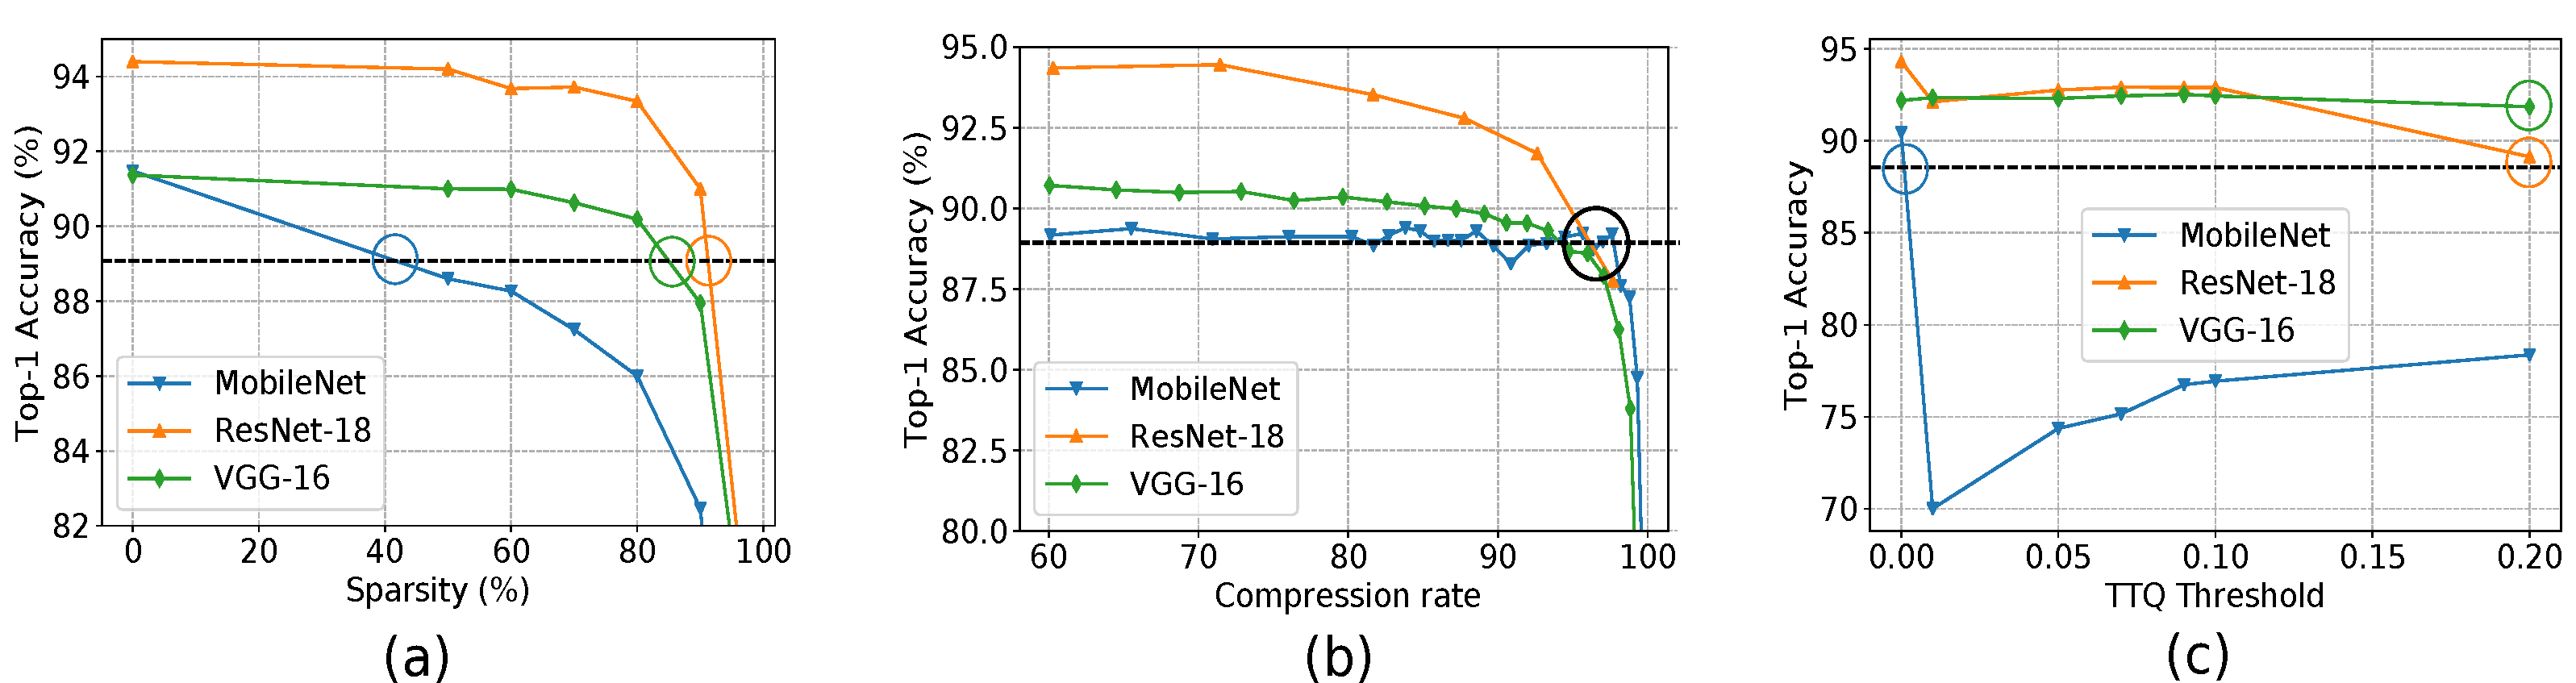
\includegraphics[width=12cm]{images/accuracy.pdf}
    \end{figure}
    
\end{frame}




\begin{frame}{Experiments}
    
    Show speed and memory requirements.
    
\end{frame}



\begin{frame}{Experiments}
    
    Show GPU results.

    
\end{frame}








\begin{frame}{Conclusion}
    
    \begin{itemize}
        \item Channel pruning is the best, always
    \end{itemize}
    
\end{frame}


\begin{frame}{Thanks}
    \begin{itemize}
        \item Bonseyes
        \item EPSRC (PPar)
    \end{itemize}
\end{frame}




\end{document}